% =====================================================================
%  Análisis de la base de datos de control robusto (DB_ssf_RS_500_c.mat)
%  Sección lista para % =====================================================================
%  Análisis de la base de datos de control robusto (DB_ssf_RS_500_c.mat)
%  Sección lista para % =====================================================================
%  Análisis de la base de datos de control robusto (DB_ssf_RS_500_c.mat)
%  Sección lista para % =====================================================================
%  Análisis de la base de datos de control robusto (DB_ssf_RS_500_c.mat)
%  Sección lista para \input{analisis_db.tex}
%  Requiere: graphicx, booktabs, amsmath, amssymb
%  \graphicspath{{figuras/}}  % o ajusta la ruta a tus figuras
% =====================================================================

\section{Caracterización de la base de datos}
\label{sec:analisis-db}

% --------------------------------------------------------------------
\subsection{Propósito y estructura}
% --------------------------------------------------------------------

La base de datos \texttt{DB\_ssf\_RS\_500\_c.mat} es el conjunto de
entrenamiento del modelo. Cada muestra describe un \emph{sistema dinámico
incierto} junto con un controlador que lo estabiliza. Conviene fijar primero la
intuición de qué es cada cosa antes de cuantificarla.

Un \textbf{sistema lineal} modela cómo evoluciona en el tiempo un vector de
estado $x(t)\in\mathbb{R}^{n_x}$ (las variables internas del proceso) cuando se
le aplica una señal de control $u(t)\in\mathbb{R}^{n_u}$:
%
\begin{equation}
  \dot{x}(t) = A\,x(t) + B\,u(t).
  \label{eq:lti}
\end{equation}
%
La matriz $A$ codifica la \emph{dinámica propia} del sistema (cómo se influyen
entre sí las variables si no hiciéramos nada), y $B$ describe \emph{cómo entra
el control} en esa dinámica. El número $n_x$ es el \emph{orden} (cuántas
variables de estado) y $n_u$ es el número de \emph{actuadores} (cuántas
perillas de control independientes hay).

En la práctica el sistema no se conoce con exactitud: hay incertidumbre en sus
parámetros. Se modela esa incertidumbre con un \textbf{politopo}, es decir, una
familia de sistemas posibles obtenida ``mezclando'' $N$ casos extremos
conocidos —los \emph{vértices} $(A_i,B_i)$— en todas las proporciones
convexas:
%
\begin{equation}
  \bigl(A(\theta),B(\theta)\bigr)=\sum_{i=1}^{N}\theta_i\,(A_i,B_i),
  \qquad \theta_i\ge 0,\ \textstyle\sum_i\theta_i=1.
  \label{eq:politopo}
\end{equation}
%
Intuitivamente, el sistema real es \emph{algún} punto dentro de la envolvente
convexa de esos $N$ vértices, pero no sabemos cuál; un controlador
\emph{robusto} debe funcionar para todos a la vez. Esto es análogo, en
términos de computación, a exigir una garantía en el \emph{peor caso} sobre un
conjunto acotado de entradas posibles.

Cada muestra de la base es por tanto una terna: el conjunto de vértices
$\{A_i\}$, el conjunto $\{B_i\}$, y una \textbf{ganancia} $K\in\mathbb{R}^{n_u\times
n_x}$ que define el controlador por realimentación de estado $u(t)=K\,x(t)$ —una
única $K$ que estabiliza todo el politopo (Tabla~\ref{tab:esquema}). La etiqueta
\texttt{RS} (\emph{robustly stabilizable}) indica que el sistema admite tal
ganancia robusta.\footnote{\textbf{Procedencia (por confirmar con el autor de la
base):} la evidencia empírica (Sec.~\ref{sec:db-control}) es consistente con que
cada $K$ se obtuvo resolviendo un problema de factibilidad (una LMI de
estabilizabilidad cuadrática), sin optimizar la rapidez de la respuesta. Falta
confirmar cómo se generaron los vértices $(A_i,B_i)$.}

\begin{table}[t]
  \centering
  \caption{Esquema de la base de datos. Cada sistema es un politopo de $N$
  vértices con una ganancia robusta $K$.}
  \label{tab:esquema}
  \begin{tabular}{llll}
    \toprule
    Campo & Símbolo & Forma & Descripción \\
    \midrule
    \texttt{A} & $\{A_i\}_{i=1}^N$ & $N\times(n_x\!\times\! n_x)$ & Dinámica propia de cada vértice \\
    \texttt{B} & $\{B_i\}_{i=1}^N$ & $N\times(n_x\!\times\! n_u)$ & Entrada de control de cada vértice \\
    \texttt{K} & $K$               & $n_u\times n_x$             & Ganancia del controlador (común) \\
    \midrule
    \multicolumn{4}{l}{$n_x\in\{2,3,4,5\}$\quad $n_u\in\{1,2\}$\quad $N\in\{2,3,4,5\}$\quad $500$ casos/celda} \\
    \bottomrule
  \end{tabular}
\end{table}

% --------------------------------------------------------------------
\subsection{Cómo se mide un sistema y su estabilidad}
\label{sec:db-conceptos}
% --------------------------------------------------------------------

Para caracterizar la base usamos un puñado de indicadores numéricos. Como el
lector no tiene por qué venir de teoría de control, los explicamos aquí en
lenguaje llano; la Tabla~\ref{tab:glosario} los resume.

\paragraph{Estabilidad y autovalores.}
La pregunta central sobre un sistema es si es \emph{estable}: si lo perturbamos,
¿vuelve al equilibrio o se dispara? Para un sistema lineal
$\dot{x}=Ax$, la respuesta la dan los \textbf{autovalores} de $A$. Toda
solución es una combinación de ``modos'' de la forma $e^{\lambda t}$, donde
$\lambda=a+bi$ es un autovalor. Su \emph{parte real} $a=\operatorname{Re}\lambda$
controla la magnitud ($e^{at}$ crece si $a>0$ y decae si $a<0$) y su parte
imaginaria $b$ controla la oscilación. Por tanto:
%
\begin{center}
  \emph{el sistema es estable} $\iff$ \emph{todos} sus autovalores cumplen
  $\operatorname{Re}\lambda<0$.
\end{center}
%
En el plano complejo, esto es ``todos los autovalores en el semiplano
izquierdo''.

\paragraph{Abscisa espectral: el modo que decide.}
No hace falta mirar todos los autovalores: basta el \emph{peor}. La
\textbf{abscisa espectral} es el mayor de las partes reales,
$\max\operatorname{Re}\lambda(A)$. Es el modo que crece más rápido (o decae más
lento) y, por sí solo, decide la estabilidad: si la abscisa es negativa, todos
los modos decaen; si es positiva, al menos uno explota. Un valor de, por
ejemplo, $832$ significa que el modo dominante crece como $e^{832\,t}$: una
inestabilidad extremadamente violenta. Lo usamos como \emph{medida relativa de
qué tan inestable} es una planta (no tiene unidades físicas porque los sistemas
son sintéticos).

\paragraph{Los dos ``máximos''.}
En las fórmulas aparecen \emph{dos} máximos anidados, y conviene separarlos:
%
\begin{equation*}
  \underbrace{\max_{i=1,\dots,N}}_{\text{(2) peor \emph{vértice}}}
  \ \underbrace{\max\,\operatorname{Re}\,\lambda(A_i)}_{\text{(1) peor \emph{modo} de ese vértice}}.
\end{equation*}
%
El máximo interno (1) recorre los autovalores de \emph{un} vértice y se queda
con su modo dominante (la abscisa espectral de $A_i$). El máximo externo (2)
recorre los $N$ vértices del politopo y se queda con el más desfavorable. La
combinación es la lectura de \emph{peor caso}: ``de toda la familia de sistemas
posibles, ¿qué tan mal se comporta el peor de ellos?''.

\paragraph{Norma de una matriz: su ``tamaño''.}
La norma espectral $\lVert A\rVert_2$ mide cuánto puede \emph{amplificar} esa
matriz a un vector (formalmente, su mayor valor singular). Es una medida del
``tamaño'' o la fuerza de la dinámica: una $\lVert A\rVert_2$ grande indica
acoplamientos internos intensos. Reportamos $\max_i\lVert A_i\rVert_2$, el
tamaño del vértice más grande del politopo.

\paragraph{Tasa de decaimiento $\alpha$: el margen de seguridad.}
Una vez cerrado el lazo con el controlador, la matriz que gobierna la dinámica
pasa a ser $A_i+B_iK$. Su abscisa espectral, cambiada de signo, es la
\textbf{tasa de decaimiento}
$\alpha=-\max_i\max\operatorname{Re}\lambda(A_i+B_iK)$. Mide \emph{qué tan
rápido} se extingue la peor respuesta: $\alpha>0$ garantiza estabilidad, y
cuanto mayor sea $\alpha$, más rápido y con más margen vuelve el sistema al
equilibrio. Un $\alpha\approx0$ significa ``estable, pero al borde'': el sistema
apenas se sostiene sobre la frontera de la inestabilidad.

\paragraph{Otros indicadores.}
La \emph{dispersión del politopo} $\max_i\lVert A_i-\bar A\rVert_2$ (con $\bar A$
el promedio de los vértices) mide qué tan distintos son los vértices entre sí,
es decir, cuánta incertidumbre hay. El \emph{número de condición} $\kappa(A_i)$
mide la sensibilidad numérica de la matriz (valores altos anticipan problemas de
precisión). El \emph{esfuerzo de control} $\lVert K\rVert_2$ mide qué tan
``agresivo'' es el controlador.

\begin{table}[t]
  \centering
  \caption{Glosario de indicadores usados en el análisis.}
  \label{tab:glosario}
  \small
  \begin{tabular}{p{3.0cm}p{3.4cm}p{6.6cm}}
    \toprule
    Indicador & En palabras simples & Un valor alto significa\dots \\
    \midrule
    Abscisa espectral (lazo abierto)\newline $\max_i\max\operatorname{Re}\lambda(A_i)$
      & Rapidez del modo más inestable del peor vértice
      & Planta muy inestable: sin control, se dispara muy rápido. \\
    Tasa de decaimiento\newline $\alpha=-\max_i\max\operatorname{Re}\lambda(A_i+B_iK)$
      & Qué tan rápido se calma el sistema ya controlado
      & Más margen de estabilidad; $\alpha\approx0$ = estable al borde. \\
    Norma $\max_i\lVert A_i\rVert_2$
      & ``Tamaño''/fuerza de la dinámica propia
      & Acoplamientos internos intensos. \\
    Norma $\max_i\lVert B_i\rVert_2$
      & Cuánto influye el control en el estado
      & Actuadores con mucha autoridad. \\
    Dispersión del politopo\newline $\max_i\lVert A_i-\bar A\rVert_2$
      & Qué tan distintos son los vértices
      & Más incertidumbre que cubrir con una sola $K$. \\
    Condición $\kappa(A_i)$
      & Sensibilidad numérica de la matriz
      & Riesgo de imprecisión numérica. \\
    Esfuerzo $\lVert K\rVert_2$
      & Qué tan ``fuerte'' es el controlador
      & Acción de control más agresiva. \\
    \bottomrule
  \end{tabular}
\end{table}

% --------------------------------------------------------------------
\subsection{Cobertura y diseño experimental}
% --------------------------------------------------------------------

El archivo organiza las muestras en un arreglo de cuatro índices,
$\texttt{BASE}[\,n_x,\,n_u,\,N,\,\text{caso}\,]$, de forma nominal
$5\times 2\times 5\times 500$. La malla está poblada parcialmente: el orden
mínimo depende del número de actuadores ($n_u{=}1\Rightarrow n_x\in\{2,\dots,5\}$;
$n_u{=}2\Rightarrow n_x\in\{3,4,5\}$) y siempre $N\ge 2$. De las $25\,000$
posiciones nominales sólo $28$ están ocupadas, con exactamente $500$ casos cada
una: en total $\mathbf{14\,000}$ sistemas ($8\,000$ con $n_u{=}1$ y $6\,000$ con
$n_u{=}2$).

La base sigue así un \emph{diseño factorial completo y perfectamente
balanceado} sobre los factores $(n_x, n_u, N)$ admisibles
(Fig.~\ref{fig:cobertura}): las $28$ combinaciones válidas aparecen con la misma
cantidad de ejemplos ($500$), sin celdas faltantes ni sobre-representadas. Este
balance es deseable para el aprendizaje: evita que el modelo privilegie una
configuración por mero desbalance de frecuencia, y permite reportar métricas
separadas por $N$ y por $n_x$ sin correcciones.

\begin{figure}[t]
  \centering
  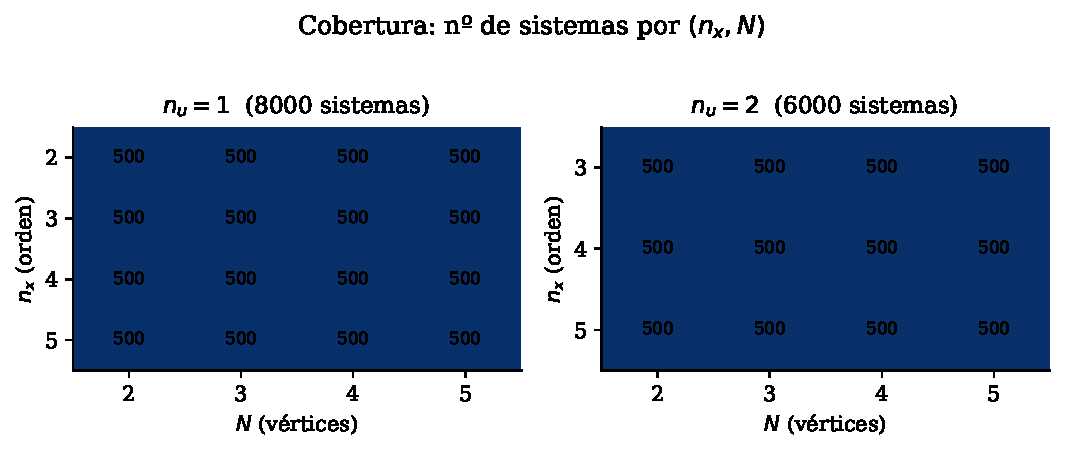
\includegraphics[width=\linewidth]{fig1_cobertura.pdf}
  \caption{Cobertura factorial: número de sistemas por $(n_x,N)$, separado por
  número de actuadores $n_u$. El soporte está completamente balanceado a $500$
  sistemas por celda.}
  \label{fig:cobertura}
\end{figure}

% --------------------------------------------------------------------
\subsection{La planta sin control (lazo abierto)}
\label{sec:db-ol}
% --------------------------------------------------------------------

``Lazo abierto'' se refiere al sistema \emph{sin} controlador. Las plantas de la
base son \emph{difíciles}: el $\mathbf{98.8\%}$ es inestable en lazo abierto
(al menos un vértice tiene un autovalor con parte real positiva), y sólo el
$1.2\%$ sería estable por sí solo. La abscisa espectral del peor vértice
(la rapidez del modo más inestable, ver Sec.~\ref{sec:db-conceptos}) tiene
mediana $30.9$ y llega hasta $\sim\!832$ (Fig.~\ref{fig:estabilidad}). En otras
palabras, la base no contiene casos triviales: el controlador debe
\emph{crear} la estabilidad, no sólo conservarla.

\begin{figure}[t]
  \centering
  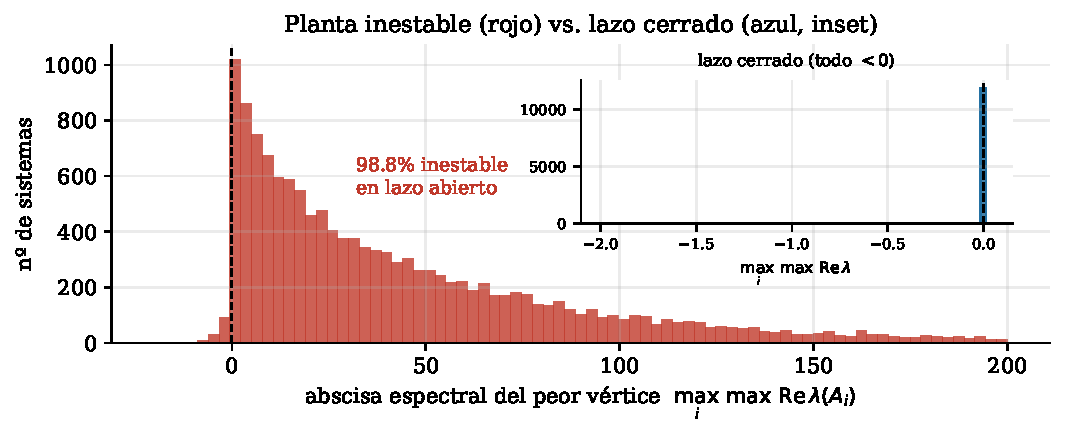
\includegraphics[width=\linewidth]{fig2_estabilidad.pdf}
  \caption{Abscisa espectral del peor vértice. Sin control la planta es
  inestable (rojo, parte real $>0$) en el $98.8\%$ de los casos; con la ganancia
  $K$ el lazo cerrado es estable en el $100\%$ (inset azul, todos $<0$).}
  \label{fig:estabilidad}
\end{figure}

En cuanto al ``tamaño'' de la dinámica (Fig.~\ref{fig:normas}), los descriptores
tienen un rango muy amplio: $\max_i\lVert A_i\rVert_2$ va de $12$ a $1012$
(mediana $131$) y crece de forma marcada con el orden $n_x$, mientras que
$\max_i\lVert B_i\rVert_2$ se mantiene acotado en $[0.74,\,16.8]$. Esta
disparidad de escalas —tres órdenes de magnitud en $\lVert A\rVert$— es
justamente la que obliga a \emph{normalizar} los datos antes de entrenar: cada
politopo se reescala dividiéndolo por su entrada de mayor magnitud,
$\gamma=\max(\max|A|,\max|B|)$, de modo que todas las cifras queden en
$[-1,1]$ y los sistemas sean comparables entre sí (esta reescala no cambia el
signo de los autovalores —y por tanto no afecta la estabilidad— aunque sí divide
la tasa de decaimiento por $\gamma$).

\begin{figure}[t]
  \centering
  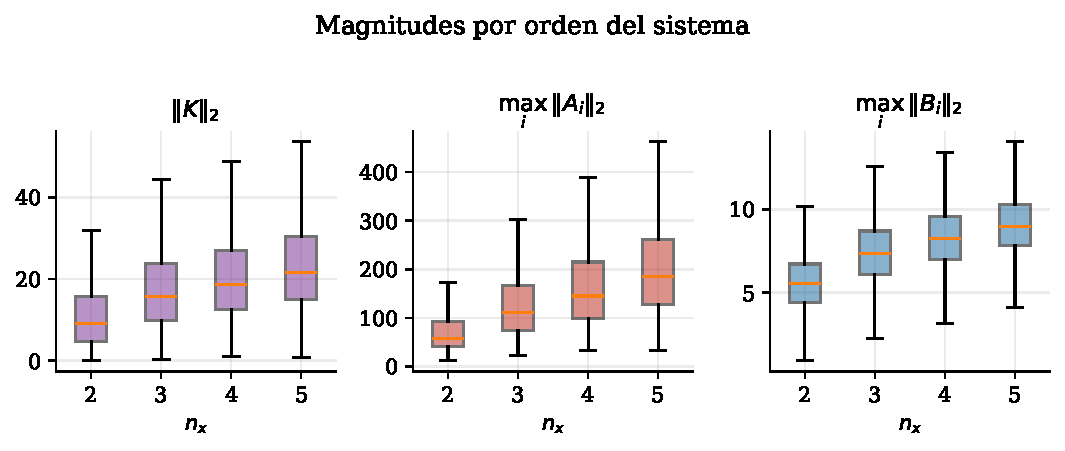
\includegraphics[width=\linewidth]{fig5_normas.pdf}
  \caption{Distribución del esfuerzo de control $\lVert K\rVert_2$ y de los
  tamaños $\max_i\lVert A_i\rVert_2$ y $\max_i\lVert B_i\rVert_2$, según el orden
  $n_x$. Ambos crecen con el orden del sistema.}
  \label{fig:normas}
\end{figure}

\paragraph{¿Se puede controlar? Controlabilidad y condicionamiento.}
Un requisito previo para que exista una ganancia estabilizante es que el sistema
sea \emph{controlable}: que desde la entrada se pueda influir en todas las
direcciones del estado. Esto se cumple en el $100\%$ de los vértices de todos
los sistemas. El número de condición de las matrices es benigno en general
($\kappa(A_i)$ con mediana $53$), con una cola pesada: un $0.39\%$ de los
sistemas supera $\kappa>10^4$, con casos extremos de hasta $5.7\times10^5$
(Fig.~\ref{fig:cond}); estos son los sistemas numéricamente delicados durante el
entrenamiento.

\begin{figure}[t]
  \centering
  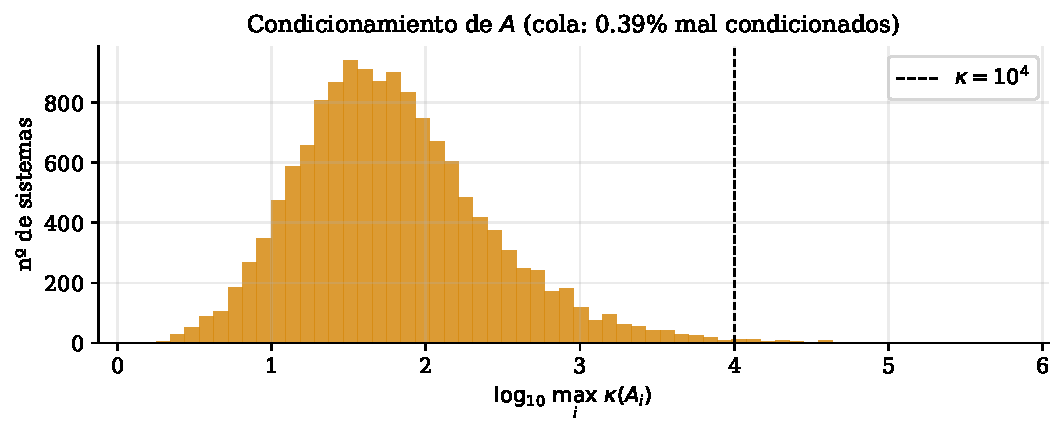
\includegraphics[width=0.82\linewidth]{fig7_condicionamiento.pdf}
  \caption{Número de condición $\max_i\kappa(A_i)$ (escala $\log_{10}$). La gran
  mayoría está bien condicionada; una cola del $0.39\%$ supera $\kappa=10^4$.}
  \label{fig:cond}
\end{figure}

% --------------------------------------------------------------------
\subsection{Tamaño de la incertidumbre (geometría del politopo)}
% --------------------------------------------------------------------

¿Qué tan ``grande'' es la incertidumbre de cada sistema? Lo medimos con la
dispersión de los vértices respecto a su promedio,
$\max_i\lVert A_i-\bar A\rVert_2$: si los vértices son muy parecidos entre sí, el
politopo es pequeño (poca incertidumbre); si son muy distintos, es grande. Su
mediana es $97.5$ y crece de forma sistemática con el número de vértices $N$
(Fig.~\ref{fig:dispersion}): más vértices implican politopos más amplios y, por
tanto, una incertidumbre más severa que la \emph{misma} ganancia $K$ debe cubrir
a la vez. Esto convierte a $N$ en un eje natural de dificultad y motiva evaluar
el modelo \emph{separado por $N$}.

\begin{figure}[t]
  \centering
  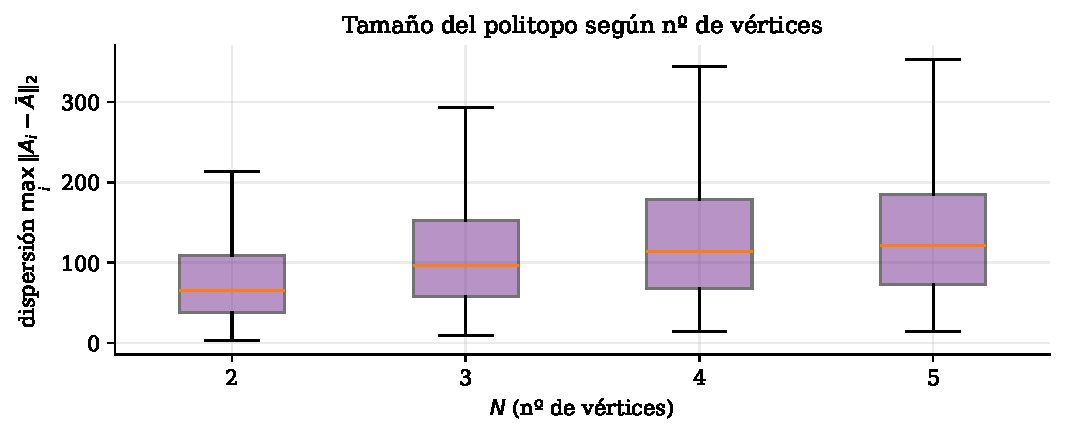
\includegraphics[width=0.82\linewidth]{fig6_dispersion.pdf}
  \caption{Tamaño del politopo $\max_i\lVert A_i-\bar A\rVert_2$ frente al número
  de vértices $N$. La incertidumbre crece con $N$.}
  \label{fig:dispersion}
\end{figure}

% --------------------------------------------------------------------
\subsection{El controlador y el sistema en lazo cerrado}
\label{sec:db-control}
% --------------------------------------------------------------------

``Lazo cerrado'' es el sistema \emph{con} el controlador conectado, gobernado por
$A_i+B_iK$. Verificamos numéricamente la etiqueta de la base recomputando los
autovalores de todos los vértices con su ganancia. El resultado es categórico:
\textbf{el $100\%$ de los $14\,000$ sistemas queda estable} (todos los
autovalores de todos los vértices con parte real negativa). No hay sistemas mal
etiquetados ni ganancias inconsistentes.

\paragraph{Estabilización ``al borde''.}
Lo más informativo es \emph{cómo} se estabiliza. La tasa de decaimiento lograda
$\alpha$ (Sec.~\ref{sec:db-conceptos}) —cuánto margen de estabilidad consigue el
controlador— se concentra masivamente junto a cero: su mediana es
$\alpha\approx 6.3\times10^{-4}$ y el $\mathbf{84.9\%}$ de los sistemas queda
\emph{casi marginal} ($\alpha<10^{-2}$), con sólo una minoría que alcanza
márgenes amplios ($\alpha_{95}=1.51$, máximo $10.6$). La distribución es
claramente \emph{bimodal} (Fig.~\ref{fig:decay}). Es decir, la ganancia de
referencia \emph{apenas} estabiliza: deja el modo dominante prácticamente sobre
la frontera de la inestabilidad.

\begin{figure}[t]
  \centering
  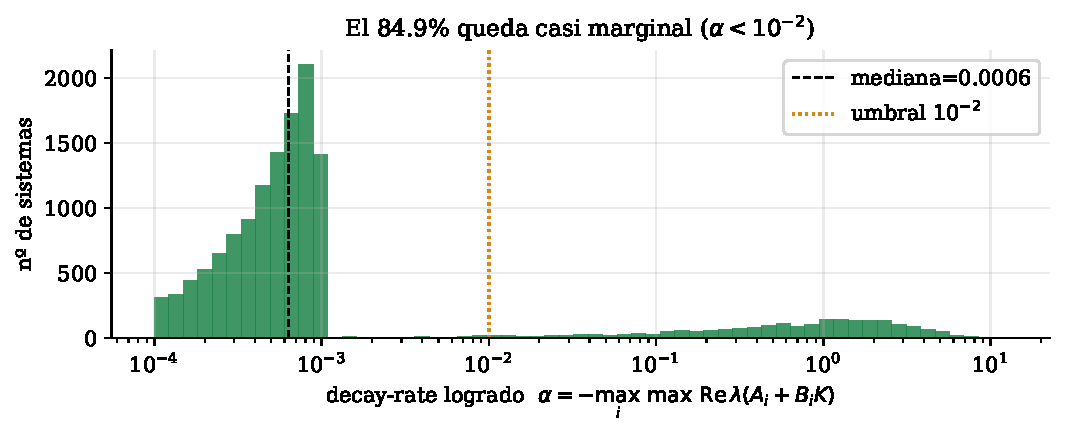
\includegraphics[width=\linewidth]{fig3_decay.pdf}
  \caption{Tasa de decaimiento lograda $\alpha$ (escala logarítmica). El
  $84.9\%$ de los sistemas queda casi marginal ($\alpha<10^{-2}$); una minoría
  exhibe márgenes grandes. La distribución es bimodal.}
  \label{fig:decay}
\end{figure}

Este comportamiento sugiere que las ganancias se construyeron buscando
\emph{cualquier} solución válida (factibilidad), no la más rápida. Lo respalda
un detalle: aunque el modo \emph{dominante} se aparca en la frontera, el resto de
los modos se empujan muy hacia la zona estable —la mediana de la parte real
sobre \emph{todos} los autovalores de lazo cerrado es $-21.4$. Visualmente, el
controlador ``refleja'' el espectro de la planta desde el semiplano inestable
(derecho) al estable (izquierdo), dejando un único modo lento que fija $\alpha$
(Fig.~\ref{fig:plano}).

\begin{figure}[t]
  \centering
  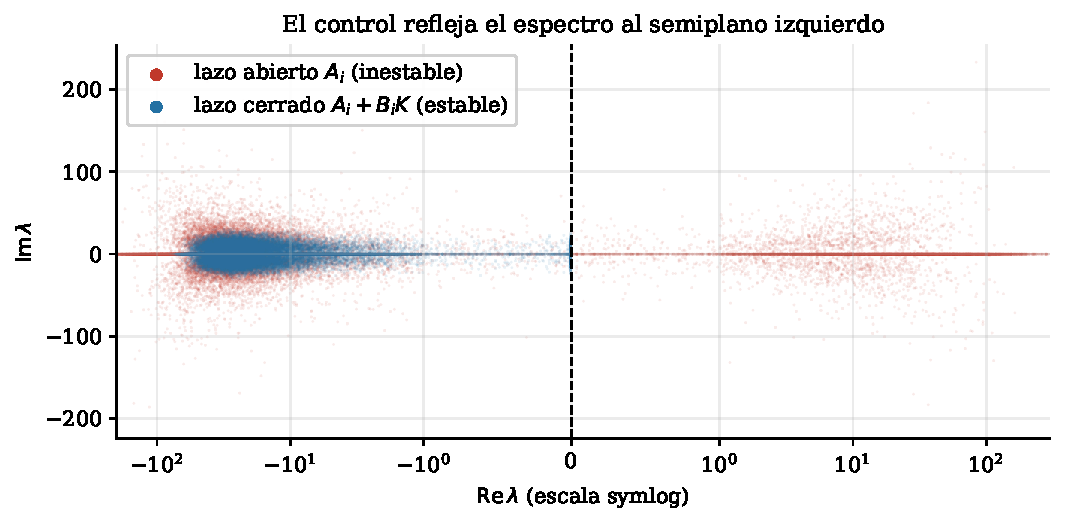
\includegraphics[width=\linewidth]{fig4_plano_complejo.pdf}
  \caption{Autovalores de los vértices en el plano complejo (eje horizontal en
  escala symlog). Sin control (rojo) la planta tiene autovalores en el semiplano
  derecho (inestables); con control (azul) todos pasan al semiplano izquierdo
  (estables), con el modo dominante pegado al eje.}
  \label{fig:plano}
\end{figure}

\paragraph{Esfuerzo de control.}
Lo ``caro'' que resulta controlar cada sistema se mide con $\lVert K\rVert_2$
(mediana $17.4$, máximo $98.1$). No es arbitrario: crece junto con el tamaño de
la planta ($\rho_{\text{Spearman}}=0.90$ frente a $\lVert A\rVert$), el tamaño
del politopo ($0.85$ frente a la dispersión) y la inestabilidad de lazo abierto
($0.63$); plantas más grandes e inestables exigen controladores más fuertes
(Fig.~\ref{fig:corr}). En cambio, la tasa de decaimiento $\alpha$ es
\emph{estadísticamente independiente} de todos los descriptores ($|\rho|\le0.04$
en todos los casos): el margen marginal no se debe a que el problema sea difícil,
sino a la forma en que se construyó la ganancia.

\begin{figure}[t]
  \centering
  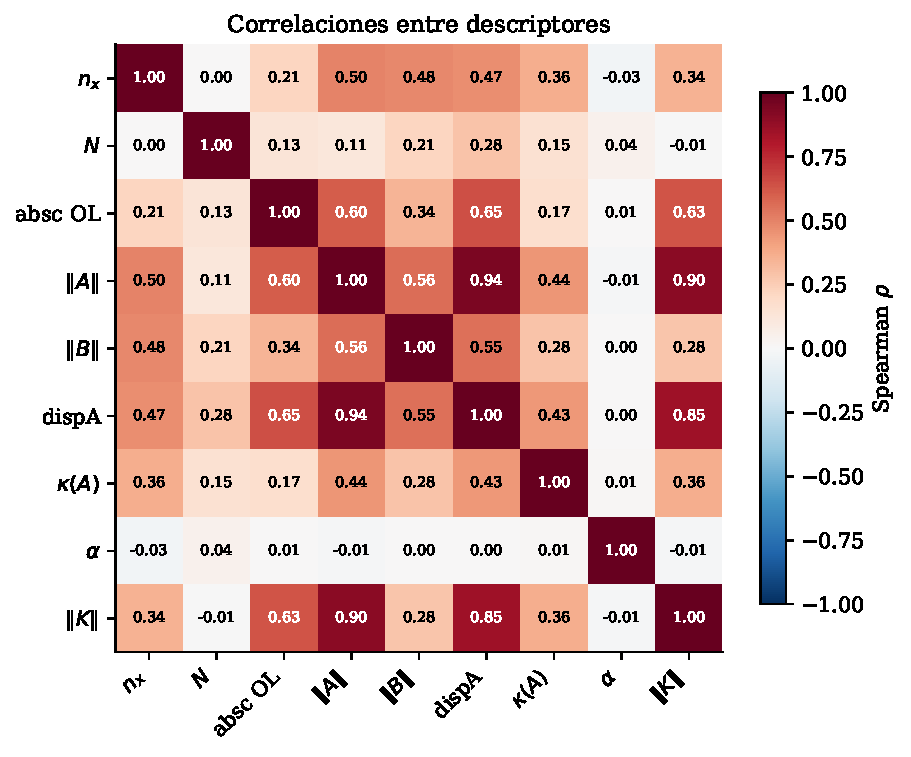
\includegraphics[width=0.78\linewidth]{fig8_correlaciones.pdf}
  \caption{Correlaciones de rango (Spearman) entre indicadores. El esfuerzo
  $\lVert K\rVert$ sigue al tamaño de la planta y del politopo; la tasa de
  decaimiento $\alpha$ no correlaciona con ningún indicador.}
  \label{fig:corr}
\end{figure}

% --------------------------------------------------------------------
\subsection{Calidad de los datos}
% --------------------------------------------------------------------

\begin{itemize}
  \item \textbf{Completitud:} sin valores faltantes en el soporte; las $28$
        celdas válidas están pobladas a $500/500$.
  \item \textbf{Validez de la etiqueta:} $100\%$ de los sistemas verificados como
        efectivamente estabilizados por su $K$ (todos los vértices estables).
  \item \textbf{Controlabilidad:} $100\%$ de los vértices controlables.
  \item \textbf{Duplicados:} no se detectaron sistemas repetidos.
  \item \textbf{Valores atípicos:} acotados y plausibles; la única cola de
        cuidado es el condicionamiento numérico ($0.39\%$ con $\kappa>10^4$),
        relevante para la estabilidad del cálculo más que para la validez del dato.
\end{itemize}

\begin{table}[t]
  \centering
  \caption{Resumen de indicadores sobre los $14\,000$ sistemas (datos crudos,
  sin normalizar).}
  \label{tab:resumen}
  \begin{tabular}{lrrr}
    \toprule
    Indicador & Mín. & Mediana & Máx. \\
    \midrule
    Abscisa espectral peor vértice (sin control) & $-17.9$ & $30.9$ & $832$ \\
    Tasa de decaimiento lograda $\alpha$         & $1.0\times10^{-4}$ & $6.3\times10^{-4}$ & $10.6$ \\
    $\max_i\lVert A_i\rVert_2$ (tamaño de la dinámica) & $12.2$ & $131$ & $1012$ \\
    $\max_i\lVert B_i\rVert_2$ (autoridad del control) & $0.74$ & $7.90$ & $16.8$ \\
    Dispersión del politopo (incertidumbre)      & $3.12$ & $97.5$ & $850$ \\
    Condición $\max_i\kappa(A_i)$                 & $1.44$ & $52.8$ & $5.7\times10^{5}$ \\
    Esfuerzo de control $\lVert K\rVert_2$        & $0.077$ & $17.4$ & $98.1$ \\
    \bottomrule
  \end{tabular}
\end{table}

% --------------------------------------------------------------------
\subsection{Implicaciones para el aprendizaje}
% --------------------------------------------------------------------

El análisis orienta varias decisiones de modelado:
%
\begin{enumerate}
  \item \textbf{Normalización imprescindible.} El rango de tamaños de $\lVert
        A\rVert$ (tres órdenes de magnitud) hace inviable alimentar las matrices
        crudas a la red; la reescala por $\gamma$ es necesaria para que el
        aprendizaje esté bien condicionado.
  \item \textbf{Invarianzas a aprovechar.} Un sistema es un \emph{conjunto} de
        vértices $\{(A_i,B_i)\}$ cuyo orden no importa y cuya cantidad $N$ varía,
        pero el certificado $K$ es común; esto motiva un codificador invariante
        al orden y a la cantidad de vértices (y, análogamente, al número de
        actuadores $n_u$).
  \item \textbf{Evaluar separado por $N$.} Como la incertidumbre crece con el
        número de vértices, conviene reportar el desempeño desglosado por $N$.
  \item \textbf{Sobre la señal de entrenamiento.} La ganancia de referencia es
        casi marginal y su $\alpha$ no aporta información sobre el sistema; esto
        respalda usar un objetivo \emph{auto-supervisado} —estabilizar con un
        margen $\alpha$ prescrito— en lugar de copiar directamente la $K$
        almacenada.
\end{enumerate}

%  Requiere: graphicx, booktabs, amsmath, amssymb
%  \graphicspath{{figuras/}}  % o ajusta la ruta a tus figuras
% =====================================================================

\section{Caracterización de la base de datos}
\label{sec:analisis-db}

% --------------------------------------------------------------------
\subsection{Propósito y estructura}
% --------------------------------------------------------------------

La base de datos \texttt{DB\_ssf\_RS\_500\_c.mat} es el conjunto de
entrenamiento del modelo. Cada muestra describe un \emph{sistema dinámico
incierto} junto con un controlador que lo estabiliza. Conviene fijar primero la
intuición de qué es cada cosa antes de cuantificarla.

Un \textbf{sistema lineal} modela cómo evoluciona en el tiempo un vector de
estado $x(t)\in\mathbb{R}^{n_x}$ (las variables internas del proceso) cuando se
le aplica una señal de control $u(t)\in\mathbb{R}^{n_u}$:
%
\begin{equation}
  \dot{x}(t) = A\,x(t) + B\,u(t).
  \label{eq:lti}
\end{equation}
%
La matriz $A$ codifica la \emph{dinámica propia} del sistema (cómo se influyen
entre sí las variables si no hiciéramos nada), y $B$ describe \emph{cómo entra
el control} en esa dinámica. El número $n_x$ es el \emph{orden} (cuántas
variables de estado) y $n_u$ es el número de \emph{actuadores} (cuántas
perillas de control independientes hay).

En la práctica el sistema no se conoce con exactitud: hay incertidumbre en sus
parámetros. Se modela esa incertidumbre con un \textbf{politopo}, es decir, una
familia de sistemas posibles obtenida ``mezclando'' $N$ casos extremos
conocidos —los \emph{vértices} $(A_i,B_i)$— en todas las proporciones
convexas:
%
\begin{equation}
  \bigl(A(\theta),B(\theta)\bigr)=\sum_{i=1}^{N}\theta_i\,(A_i,B_i),
  \qquad \theta_i\ge 0,\ \textstyle\sum_i\theta_i=1.
  \label{eq:politopo}
\end{equation}
%
Intuitivamente, el sistema real es \emph{algún} punto dentro de la envolvente
convexa de esos $N$ vértices, pero no sabemos cuál; un controlador
\emph{robusto} debe funcionar para todos a la vez. Esto es análogo, en
términos de computación, a exigir una garantía en el \emph{peor caso} sobre un
conjunto acotado de entradas posibles.

Cada muestra de la base es por tanto una terna: el conjunto de vértices
$\{A_i\}$, el conjunto $\{B_i\}$, y una \textbf{ganancia} $K\in\mathbb{R}^{n_u\times
n_x}$ que define el controlador por realimentación de estado $u(t)=K\,x(t)$ —una
única $K$ que estabiliza todo el politopo (Tabla~\ref{tab:esquema}). La etiqueta
\texttt{RS} (\emph{robustly stabilizable}) indica que el sistema admite tal
ganancia robusta.\footnote{\textbf{Procedencia (por confirmar con el autor de la
base):} la evidencia empírica (Sec.~\ref{sec:db-control}) es consistente con que
cada $K$ se obtuvo resolviendo un problema de factibilidad (una LMI de
estabilizabilidad cuadrática), sin optimizar la rapidez de la respuesta. Falta
confirmar cómo se generaron los vértices $(A_i,B_i)$.}

\begin{table}[t]
  \centering
  \caption{Esquema de la base de datos. Cada sistema es un politopo de $N$
  vértices con una ganancia robusta $K$.}
  \label{tab:esquema}
  \begin{tabular}{llll}
    \toprule
    Campo & Símbolo & Forma & Descripción \\
    \midrule
    \texttt{A} & $\{A_i\}_{i=1}^N$ & $N\times(n_x\!\times\! n_x)$ & Dinámica propia de cada vértice \\
    \texttt{B} & $\{B_i\}_{i=1}^N$ & $N\times(n_x\!\times\! n_u)$ & Entrada de control de cada vértice \\
    \texttt{K} & $K$               & $n_u\times n_x$             & Ganancia del controlador (común) \\
    \midrule
    \multicolumn{4}{l}{$n_x\in\{2,3,4,5\}$\quad $n_u\in\{1,2\}$\quad $N\in\{2,3,4,5\}$\quad $500$ casos/celda} \\
    \bottomrule
  \end{tabular}
\end{table}

% --------------------------------------------------------------------
\subsection{Cómo se mide un sistema y su estabilidad}
\label{sec:db-conceptos}
% --------------------------------------------------------------------

Para caracterizar la base usamos un puñado de indicadores numéricos. Como el
lector no tiene por qué venir de teoría de control, los explicamos aquí en
lenguaje llano; la Tabla~\ref{tab:glosario} los resume.

\paragraph{Estabilidad y autovalores.}
La pregunta central sobre un sistema es si es \emph{estable}: si lo perturbamos,
¿vuelve al equilibrio o se dispara? Para un sistema lineal
$\dot{x}=Ax$, la respuesta la dan los \textbf{autovalores} de $A$. Toda
solución es una combinación de ``modos'' de la forma $e^{\lambda t}$, donde
$\lambda=a+bi$ es un autovalor. Su \emph{parte real} $a=\operatorname{Re}\lambda$
controla la magnitud ($e^{at}$ crece si $a>0$ y decae si $a<0$) y su parte
imaginaria $b$ controla la oscilación. Por tanto:
%
\begin{center}
  \emph{el sistema es estable} $\iff$ \emph{todos} sus autovalores cumplen
  $\operatorname{Re}\lambda<0$.
\end{center}
%
En el plano complejo, esto es ``todos los autovalores en el semiplano
izquierdo''.

\paragraph{Abscisa espectral: el modo que decide.}
No hace falta mirar todos los autovalores: basta el \emph{peor}. La
\textbf{abscisa espectral} es el mayor de las partes reales,
$\max\operatorname{Re}\lambda(A)$. Es el modo que crece más rápido (o decae más
lento) y, por sí solo, decide la estabilidad: si la abscisa es negativa, todos
los modos decaen; si es positiva, al menos uno explota. Un valor de, por
ejemplo, $832$ significa que el modo dominante crece como $e^{832\,t}$: una
inestabilidad extremadamente violenta. Lo usamos como \emph{medida relativa de
qué tan inestable} es una planta (no tiene unidades físicas porque los sistemas
son sintéticos).

\paragraph{Los dos ``máximos''.}
En las fórmulas aparecen \emph{dos} máximos anidados, y conviene separarlos:
%
\begin{equation*}
  \underbrace{\max_{i=1,\dots,N}}_{\text{(2) peor \emph{vértice}}}
  \ \underbrace{\max\,\operatorname{Re}\,\lambda(A_i)}_{\text{(1) peor \emph{modo} de ese vértice}}.
\end{equation*}
%
El máximo interno (1) recorre los autovalores de \emph{un} vértice y se queda
con su modo dominante (la abscisa espectral de $A_i$). El máximo externo (2)
recorre los $N$ vértices del politopo y se queda con el más desfavorable. La
combinación es la lectura de \emph{peor caso}: ``de toda la familia de sistemas
posibles, ¿qué tan mal se comporta el peor de ellos?''.

\paragraph{Norma de una matriz: su ``tamaño''.}
La norma espectral $\lVert A\rVert_2$ mide cuánto puede \emph{amplificar} esa
matriz a un vector (formalmente, su mayor valor singular). Es una medida del
``tamaño'' o la fuerza de la dinámica: una $\lVert A\rVert_2$ grande indica
acoplamientos internos intensos. Reportamos $\max_i\lVert A_i\rVert_2$, el
tamaño del vértice más grande del politopo.

\paragraph{Tasa de decaimiento $\alpha$: el margen de seguridad.}
Una vez cerrado el lazo con el controlador, la matriz que gobierna la dinámica
pasa a ser $A_i+B_iK$. Su abscisa espectral, cambiada de signo, es la
\textbf{tasa de decaimiento}
$\alpha=-\max_i\max\operatorname{Re}\lambda(A_i+B_iK)$. Mide \emph{qué tan
rápido} se extingue la peor respuesta: $\alpha>0$ garantiza estabilidad, y
cuanto mayor sea $\alpha$, más rápido y con más margen vuelve el sistema al
equilibrio. Un $\alpha\approx0$ significa ``estable, pero al borde'': el sistema
apenas se sostiene sobre la frontera de la inestabilidad.

\paragraph{Otros indicadores.}
La \emph{dispersión del politopo} $\max_i\lVert A_i-\bar A\rVert_2$ (con $\bar A$
el promedio de los vértices) mide qué tan distintos son los vértices entre sí,
es decir, cuánta incertidumbre hay. El \emph{número de condición} $\kappa(A_i)$
mide la sensibilidad numérica de la matriz (valores altos anticipan problemas de
precisión). El \emph{esfuerzo de control} $\lVert K\rVert_2$ mide qué tan
``agresivo'' es el controlador.

\begin{table}[t]
  \centering
  \caption{Glosario de indicadores usados en el análisis.}
  \label{tab:glosario}
  \small
  \begin{tabular}{p{3.0cm}p{3.4cm}p{6.6cm}}
    \toprule
    Indicador & En palabras simples & Un valor alto significa\dots \\
    \midrule
    Abscisa espectral (lazo abierto)\newline $\max_i\max\operatorname{Re}\lambda(A_i)$
      & Rapidez del modo más inestable del peor vértice
      & Planta muy inestable: sin control, se dispara muy rápido. \\
    Tasa de decaimiento\newline $\alpha=-\max_i\max\operatorname{Re}\lambda(A_i+B_iK)$
      & Qué tan rápido se calma el sistema ya controlado
      & Más margen de estabilidad; $\alpha\approx0$ = estable al borde. \\
    Norma $\max_i\lVert A_i\rVert_2$
      & ``Tamaño''/fuerza de la dinámica propia
      & Acoplamientos internos intensos. \\
    Norma $\max_i\lVert B_i\rVert_2$
      & Cuánto influye el control en el estado
      & Actuadores con mucha autoridad. \\
    Dispersión del politopo\newline $\max_i\lVert A_i-\bar A\rVert_2$
      & Qué tan distintos son los vértices
      & Más incertidumbre que cubrir con una sola $K$. \\
    Condición $\kappa(A_i)$
      & Sensibilidad numérica de la matriz
      & Riesgo de imprecisión numérica. \\
    Esfuerzo $\lVert K\rVert_2$
      & Qué tan ``fuerte'' es el controlador
      & Acción de control más agresiva. \\
    \bottomrule
  \end{tabular}
\end{table}

% --------------------------------------------------------------------
\subsection{Cobertura y diseño experimental}
% --------------------------------------------------------------------

El archivo organiza las muestras en un arreglo de cuatro índices,
$\texttt{BASE}[\,n_x,\,n_u,\,N,\,\text{caso}\,]$, de forma nominal
$5\times 2\times 5\times 500$. La malla está poblada parcialmente: el orden
mínimo depende del número de actuadores ($n_u{=}1\Rightarrow n_x\in\{2,\dots,5\}$;
$n_u{=}2\Rightarrow n_x\in\{3,4,5\}$) y siempre $N\ge 2$. De las $25\,000$
posiciones nominales sólo $28$ están ocupadas, con exactamente $500$ casos cada
una: en total $\mathbf{14\,000}$ sistemas ($8\,000$ con $n_u{=}1$ y $6\,000$ con
$n_u{=}2$).

La base sigue así un \emph{diseño factorial completo y perfectamente
balanceado} sobre los factores $(n_x, n_u, N)$ admisibles
(Fig.~\ref{fig:cobertura}): las $28$ combinaciones válidas aparecen con la misma
cantidad de ejemplos ($500$), sin celdas faltantes ni sobre-representadas. Este
balance es deseable para el aprendizaje: evita que el modelo privilegie una
configuración por mero desbalance de frecuencia, y permite reportar métricas
separadas por $N$ y por $n_x$ sin correcciones.

\begin{figure}[t]
  \centering
  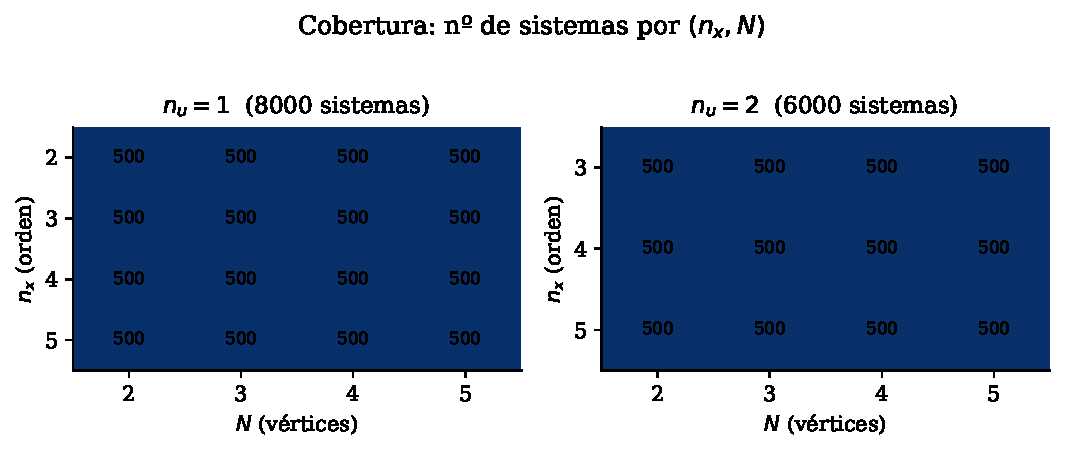
\includegraphics[width=\linewidth]{fig1_cobertura.pdf}
  \caption{Cobertura factorial: número de sistemas por $(n_x,N)$, separado por
  número de actuadores $n_u$. El soporte está completamente balanceado a $500$
  sistemas por celda.}
  \label{fig:cobertura}
\end{figure}

% --------------------------------------------------------------------
\subsection{La planta sin control (lazo abierto)}
\label{sec:db-ol}
% --------------------------------------------------------------------

``Lazo abierto'' se refiere al sistema \emph{sin} controlador. Las plantas de la
base son \emph{difíciles}: el $\mathbf{98.8\%}$ es inestable en lazo abierto
(al menos un vértice tiene un autovalor con parte real positiva), y sólo el
$1.2\%$ sería estable por sí solo. La abscisa espectral del peor vértice
(la rapidez del modo más inestable, ver Sec.~\ref{sec:db-conceptos}) tiene
mediana $30.9$ y llega hasta $\sim\!832$ (Fig.~\ref{fig:estabilidad}). En otras
palabras, la base no contiene casos triviales: el controlador debe
\emph{crear} la estabilidad, no sólo conservarla.

\begin{figure}[t]
  \centering
  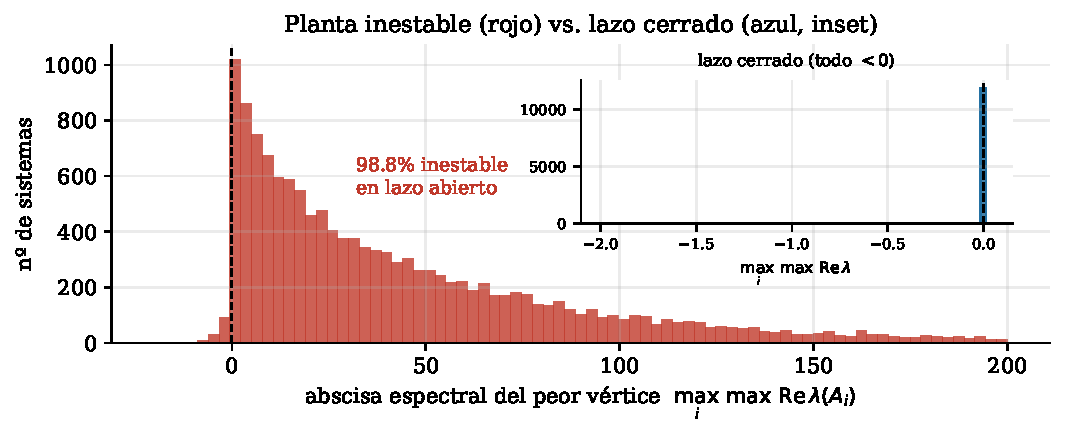
\includegraphics[width=\linewidth]{fig2_estabilidad.pdf}
  \caption{Abscisa espectral del peor vértice. Sin control la planta es
  inestable (rojo, parte real $>0$) en el $98.8\%$ de los casos; con la ganancia
  $K$ el lazo cerrado es estable en el $100\%$ (inset azul, todos $<0$).}
  \label{fig:estabilidad}
\end{figure}

En cuanto al ``tamaño'' de la dinámica (Fig.~\ref{fig:normas}), los descriptores
tienen un rango muy amplio: $\max_i\lVert A_i\rVert_2$ va de $12$ a $1012$
(mediana $131$) y crece de forma marcada con el orden $n_x$, mientras que
$\max_i\lVert B_i\rVert_2$ se mantiene acotado en $[0.74,\,16.8]$. Esta
disparidad de escalas —tres órdenes de magnitud en $\lVert A\rVert$— es
justamente la que obliga a \emph{normalizar} los datos antes de entrenar: cada
politopo se reescala dividiéndolo por su entrada de mayor magnitud,
$\gamma=\max(\max|A|,\max|B|)$, de modo que todas las cifras queden en
$[-1,1]$ y los sistemas sean comparables entre sí (esta reescala no cambia el
signo de los autovalores —y por tanto no afecta la estabilidad— aunque sí divide
la tasa de decaimiento por $\gamma$).

\begin{figure}[t]
  \centering
  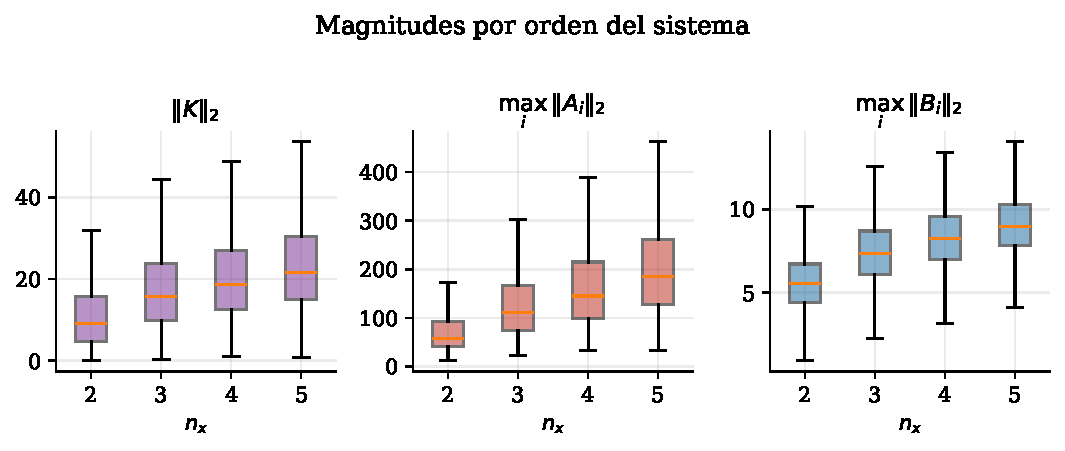
\includegraphics[width=\linewidth]{fig5_normas.pdf}
  \caption{Distribución del esfuerzo de control $\lVert K\rVert_2$ y de los
  tamaños $\max_i\lVert A_i\rVert_2$ y $\max_i\lVert B_i\rVert_2$, según el orden
  $n_x$. Ambos crecen con el orden del sistema.}
  \label{fig:normas}
\end{figure}

\paragraph{¿Se puede controlar? Controlabilidad y condicionamiento.}
Un requisito previo para que exista una ganancia estabilizante es que el sistema
sea \emph{controlable}: que desde la entrada se pueda influir en todas las
direcciones del estado. Esto se cumple en el $100\%$ de los vértices de todos
los sistemas. El número de condición de las matrices es benigno en general
($\kappa(A_i)$ con mediana $53$), con una cola pesada: un $0.39\%$ de los
sistemas supera $\kappa>10^4$, con casos extremos de hasta $5.7\times10^5$
(Fig.~\ref{fig:cond}); estos son los sistemas numéricamente delicados durante el
entrenamiento.

\begin{figure}[t]
  \centering
  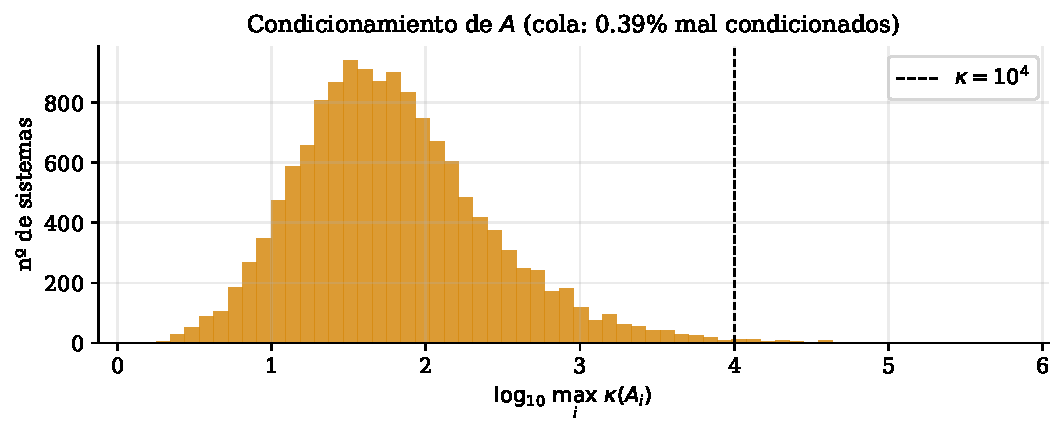
\includegraphics[width=0.82\linewidth]{fig7_condicionamiento.pdf}
  \caption{Número de condición $\max_i\kappa(A_i)$ (escala $\log_{10}$). La gran
  mayoría está bien condicionada; una cola del $0.39\%$ supera $\kappa=10^4$.}
  \label{fig:cond}
\end{figure}

% --------------------------------------------------------------------
\subsection{Tamaño de la incertidumbre (geometría del politopo)}
% --------------------------------------------------------------------

¿Qué tan ``grande'' es la incertidumbre de cada sistema? Lo medimos con la
dispersión de los vértices respecto a su promedio,
$\max_i\lVert A_i-\bar A\rVert_2$: si los vértices son muy parecidos entre sí, el
politopo es pequeño (poca incertidumbre); si son muy distintos, es grande. Su
mediana es $97.5$ y crece de forma sistemática con el número de vértices $N$
(Fig.~\ref{fig:dispersion}): más vértices implican politopos más amplios y, por
tanto, una incertidumbre más severa que la \emph{misma} ganancia $K$ debe cubrir
a la vez. Esto convierte a $N$ en un eje natural de dificultad y motiva evaluar
el modelo \emph{separado por $N$}.

\begin{figure}[t]
  \centering
  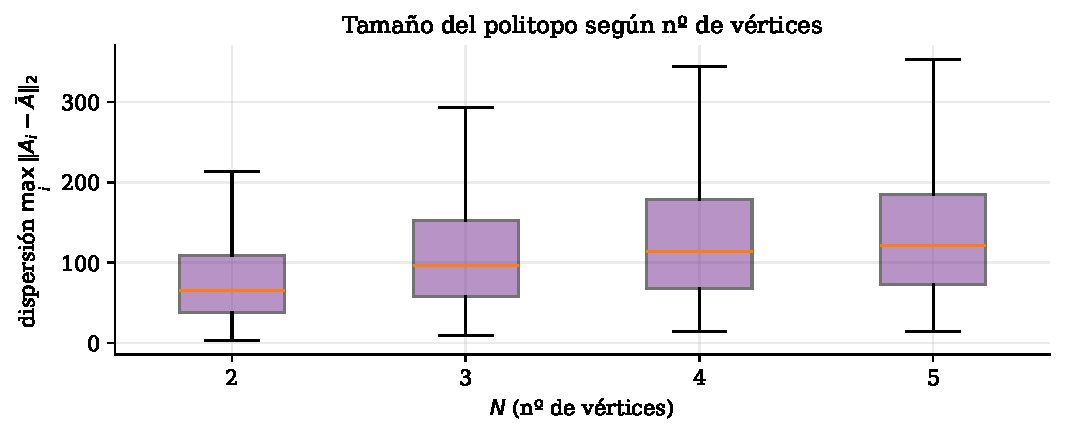
\includegraphics[width=0.82\linewidth]{fig6_dispersion.pdf}
  \caption{Tamaño del politopo $\max_i\lVert A_i-\bar A\rVert_2$ frente al número
  de vértices $N$. La incertidumbre crece con $N$.}
  \label{fig:dispersion}
\end{figure}

% --------------------------------------------------------------------
\subsection{El controlador y el sistema en lazo cerrado}
\label{sec:db-control}
% --------------------------------------------------------------------

``Lazo cerrado'' es el sistema \emph{con} el controlador conectado, gobernado por
$A_i+B_iK$. Verificamos numéricamente la etiqueta de la base recomputando los
autovalores de todos los vértices con su ganancia. El resultado es categórico:
\textbf{el $100\%$ de los $14\,000$ sistemas queda estable} (todos los
autovalores de todos los vértices con parte real negativa). No hay sistemas mal
etiquetados ni ganancias inconsistentes.

\paragraph{Estabilización ``al borde''.}
Lo más informativo es \emph{cómo} se estabiliza. La tasa de decaimiento lograda
$\alpha$ (Sec.~\ref{sec:db-conceptos}) —cuánto margen de estabilidad consigue el
controlador— se concentra masivamente junto a cero: su mediana es
$\alpha\approx 6.3\times10^{-4}$ y el $\mathbf{84.9\%}$ de los sistemas queda
\emph{casi marginal} ($\alpha<10^{-2}$), con sólo una minoría que alcanza
márgenes amplios ($\alpha_{95}=1.51$, máximo $10.6$). La distribución es
claramente \emph{bimodal} (Fig.~\ref{fig:decay}). Es decir, la ganancia de
referencia \emph{apenas} estabiliza: deja el modo dominante prácticamente sobre
la frontera de la inestabilidad.

\begin{figure}[t]
  \centering
  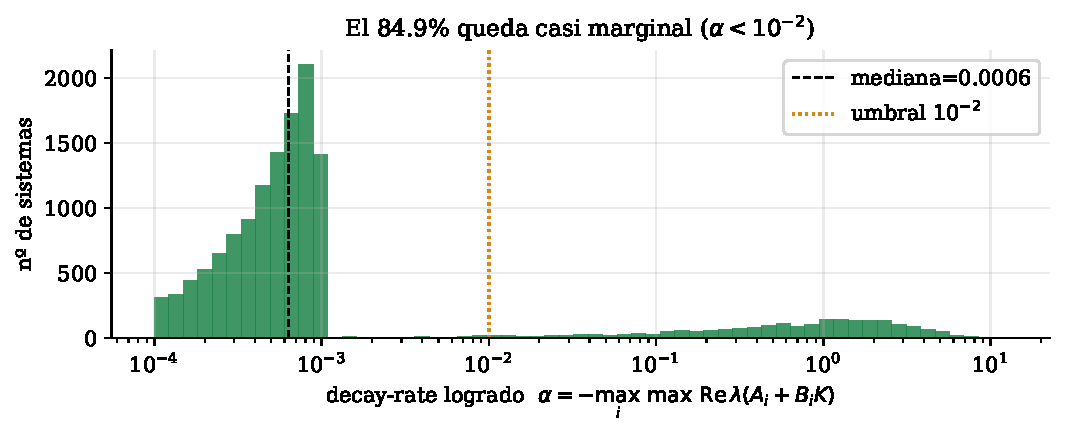
\includegraphics[width=\linewidth]{fig3_decay.pdf}
  \caption{Tasa de decaimiento lograda $\alpha$ (escala logarítmica). El
  $84.9\%$ de los sistemas queda casi marginal ($\alpha<10^{-2}$); una minoría
  exhibe márgenes grandes. La distribución es bimodal.}
  \label{fig:decay}
\end{figure}

Este comportamiento sugiere que las ganancias se construyeron buscando
\emph{cualquier} solución válida (factibilidad), no la más rápida. Lo respalda
un detalle: aunque el modo \emph{dominante} se aparca en la frontera, el resto de
los modos se empujan muy hacia la zona estable —la mediana de la parte real
sobre \emph{todos} los autovalores de lazo cerrado es $-21.4$. Visualmente, el
controlador ``refleja'' el espectro de la planta desde el semiplano inestable
(derecho) al estable (izquierdo), dejando un único modo lento que fija $\alpha$
(Fig.~\ref{fig:plano}).

\begin{figure}[t]
  \centering
  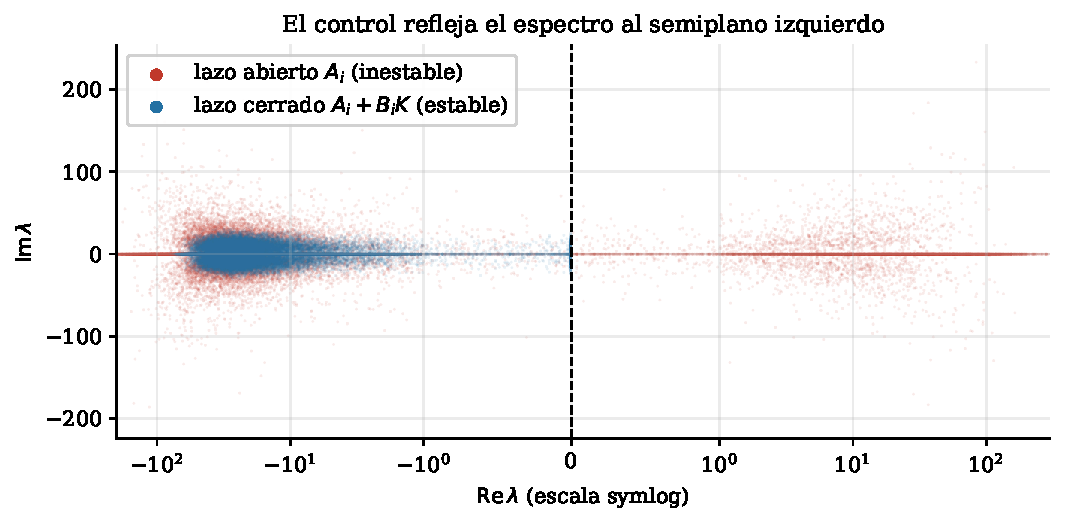
\includegraphics[width=\linewidth]{fig4_plano_complejo.pdf}
  \caption{Autovalores de los vértices en el plano complejo (eje horizontal en
  escala symlog). Sin control (rojo) la planta tiene autovalores en el semiplano
  derecho (inestables); con control (azul) todos pasan al semiplano izquierdo
  (estables), con el modo dominante pegado al eje.}
  \label{fig:plano}
\end{figure}

\paragraph{Esfuerzo de control.}
Lo ``caro'' que resulta controlar cada sistema se mide con $\lVert K\rVert_2$
(mediana $17.4$, máximo $98.1$). No es arbitrario: crece junto con el tamaño de
la planta ($\rho_{\text{Spearman}}=0.90$ frente a $\lVert A\rVert$), el tamaño
del politopo ($0.85$ frente a la dispersión) y la inestabilidad de lazo abierto
($0.63$); plantas más grandes e inestables exigen controladores más fuertes
(Fig.~\ref{fig:corr}). En cambio, la tasa de decaimiento $\alpha$ es
\emph{estadísticamente independiente} de todos los descriptores ($|\rho|\le0.04$
en todos los casos): el margen marginal no se debe a que el problema sea difícil,
sino a la forma en que se construyó la ganancia.

\begin{figure}[t]
  \centering
  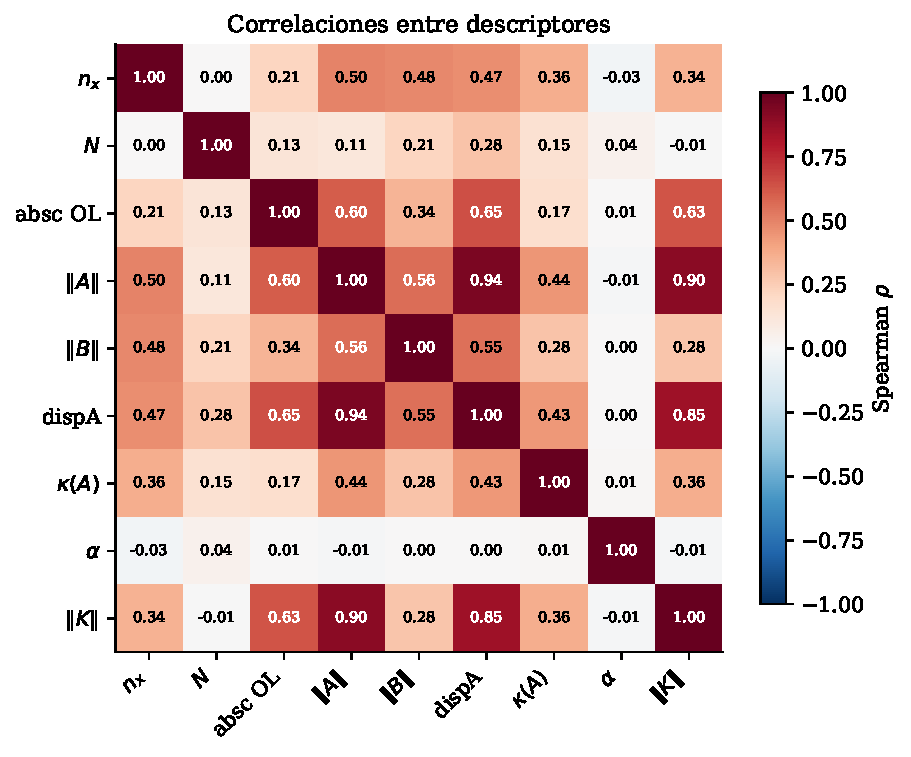
\includegraphics[width=0.78\linewidth]{fig8_correlaciones.pdf}
  \caption{Correlaciones de rango (Spearman) entre indicadores. El esfuerzo
  $\lVert K\rVert$ sigue al tamaño de la planta y del politopo; la tasa de
  decaimiento $\alpha$ no correlaciona con ningún indicador.}
  \label{fig:corr}
\end{figure}

% --------------------------------------------------------------------
\subsection{Calidad de los datos}
% --------------------------------------------------------------------

\begin{itemize}
  \item \textbf{Completitud:} sin valores faltantes en el soporte; las $28$
        celdas válidas están pobladas a $500/500$.
  \item \textbf{Validez de la etiqueta:} $100\%$ de los sistemas verificados como
        efectivamente estabilizados por su $K$ (todos los vértices estables).
  \item \textbf{Controlabilidad:} $100\%$ de los vértices controlables.
  \item \textbf{Duplicados:} no se detectaron sistemas repetidos.
  \item \textbf{Valores atípicos:} acotados y plausibles; la única cola de
        cuidado es el condicionamiento numérico ($0.39\%$ con $\kappa>10^4$),
        relevante para la estabilidad del cálculo más que para la validez del dato.
\end{itemize}

\begin{table}[t]
  \centering
  \caption{Resumen de indicadores sobre los $14\,000$ sistemas (datos crudos,
  sin normalizar).}
  \label{tab:resumen}
  \begin{tabular}{lrrr}
    \toprule
    Indicador & Mín. & Mediana & Máx. \\
    \midrule
    Abscisa espectral peor vértice (sin control) & $-17.9$ & $30.9$ & $832$ \\
    Tasa de decaimiento lograda $\alpha$         & $1.0\times10^{-4}$ & $6.3\times10^{-4}$ & $10.6$ \\
    $\max_i\lVert A_i\rVert_2$ (tamaño de la dinámica) & $12.2$ & $131$ & $1012$ \\
    $\max_i\lVert B_i\rVert_2$ (autoridad del control) & $0.74$ & $7.90$ & $16.8$ \\
    Dispersión del politopo (incertidumbre)      & $3.12$ & $97.5$ & $850$ \\
    Condición $\max_i\kappa(A_i)$                 & $1.44$ & $52.8$ & $5.7\times10^{5}$ \\
    Esfuerzo de control $\lVert K\rVert_2$        & $0.077$ & $17.4$ & $98.1$ \\
    \bottomrule
  \end{tabular}
\end{table}

% --------------------------------------------------------------------
\subsection{Implicaciones para el aprendizaje}
% --------------------------------------------------------------------

El análisis orienta varias decisiones de modelado:
%
\begin{enumerate}
  \item \textbf{Normalización imprescindible.} El rango de tamaños de $\lVert
        A\rVert$ (tres órdenes de magnitud) hace inviable alimentar las matrices
        crudas a la red; la reescala por $\gamma$ es necesaria para que el
        aprendizaje esté bien condicionado.
  \item \textbf{Invarianzas a aprovechar.} Un sistema es un \emph{conjunto} de
        vértices $\{(A_i,B_i)\}$ cuyo orden no importa y cuya cantidad $N$ varía,
        pero el certificado $K$ es común; esto motiva un codificador invariante
        al orden y a la cantidad de vértices (y, análogamente, al número de
        actuadores $n_u$).
  \item \textbf{Evaluar separado por $N$.} Como la incertidumbre crece con el
        número de vértices, conviene reportar el desempeño desglosado por $N$.
  \item \textbf{Sobre la señal de entrenamiento.} La ganancia de referencia es
        casi marginal y su $\alpha$ no aporta información sobre el sistema; esto
        respalda usar un objetivo \emph{auto-supervisado} —estabilizar con un
        margen $\alpha$ prescrito— en lugar de copiar directamente la $K$
        almacenada.
\end{enumerate}

%  Requiere: graphicx, booktabs, amsmath, amssymb
%  \graphicspath{{figuras/}}  % o ajusta la ruta a tus figuras
% =====================================================================

\section{Caracterización de la base de datos}
\label{sec:analisis-db}

% --------------------------------------------------------------------
\subsection{Propósito y estructura}
% --------------------------------------------------------------------

La base de datos \texttt{DB\_ssf\_RS\_500\_c.mat} es el conjunto de
entrenamiento del modelo. Cada muestra describe un \emph{sistema dinámico
incierto} junto con un controlador que lo estabiliza. Conviene fijar primero la
intuición de qué es cada cosa antes de cuantificarla.

Un \textbf{sistema lineal} modela cómo evoluciona en el tiempo un vector de
estado $x(t)\in\mathbb{R}^{n_x}$ (las variables internas del proceso) cuando se
le aplica una señal de control $u(t)\in\mathbb{R}^{n_u}$:
%
\begin{equation}
  \dot{x}(t) = A\,x(t) + B\,u(t).
  \label{eq:lti}
\end{equation}
%
La matriz $A$ codifica la \emph{dinámica propia} del sistema (cómo se influyen
entre sí las variables si no hiciéramos nada), y $B$ describe \emph{cómo entra
el control} en esa dinámica. El número $n_x$ es el \emph{orden} (cuántas
variables de estado) y $n_u$ es el número de \emph{actuadores} (cuántas
perillas de control independientes hay).

En la práctica el sistema no se conoce con exactitud: hay incertidumbre en sus
parámetros. Se modela esa incertidumbre con un \textbf{politopo}, es decir, una
familia de sistemas posibles obtenida ``mezclando'' $N$ casos extremos
conocidos —los \emph{vértices} $(A_i,B_i)$— en todas las proporciones
convexas:
%
\begin{equation}
  \bigl(A(\theta),B(\theta)\bigr)=\sum_{i=1}^{N}\theta_i\,(A_i,B_i),
  \qquad \theta_i\ge 0,\ \textstyle\sum_i\theta_i=1.
  \label{eq:politopo}
\end{equation}
%
Intuitivamente, el sistema real es \emph{algún} punto dentro de la envolvente
convexa de esos $N$ vértices, pero no sabemos cuál; un controlador
\emph{robusto} debe funcionar para todos a la vez. Esto es análogo, en
términos de computación, a exigir una garantía en el \emph{peor caso} sobre un
conjunto acotado de entradas posibles.

Cada muestra de la base es por tanto una terna: el conjunto de vértices
$\{A_i\}$, el conjunto $\{B_i\}$, y una \textbf{ganancia} $K\in\mathbb{R}^{n_u\times
n_x}$ que define el controlador por realimentación de estado $u(t)=K\,x(t)$ —una
única $K$ que estabiliza todo el politopo (Tabla~\ref{tab:esquema}). La etiqueta
\texttt{RS} (\emph{robustly stabilizable}) indica que el sistema admite tal
ganancia robusta.\footnote{\textbf{Procedencia (por confirmar con el autor de la
base):} la evidencia empírica (Sec.~\ref{sec:db-control}) es consistente con que
cada $K$ se obtuvo resolviendo un problema de factibilidad (una LMI de
estabilizabilidad cuadrática), sin optimizar la rapidez de la respuesta. Falta
confirmar cómo se generaron los vértices $(A_i,B_i)$.}

\begin{table}[t]
  \centering
  \caption{Esquema de la base de datos. Cada sistema es un politopo de $N$
  vértices con una ganancia robusta $K$.}
  \label{tab:esquema}
  \begin{tabular}{llll}
    \toprule
    Campo & Símbolo & Forma & Descripción \\
    \midrule
    \texttt{A} & $\{A_i\}_{i=1}^N$ & $N\times(n_x\!\times\! n_x)$ & Dinámica propia de cada vértice \\
    \texttt{B} & $\{B_i\}_{i=1}^N$ & $N\times(n_x\!\times\! n_u)$ & Entrada de control de cada vértice \\
    \texttt{K} & $K$               & $n_u\times n_x$             & Ganancia del controlador (común) \\
    \midrule
    \multicolumn{4}{l}{$n_x\in\{2,3,4,5\}$\quad $n_u\in\{1,2\}$\quad $N\in\{2,3,4,5\}$\quad $500$ casos/celda} \\
    \bottomrule
  \end{tabular}
\end{table}

% --------------------------------------------------------------------
\subsection{Cómo se mide un sistema y su estabilidad}
\label{sec:db-conceptos}
% --------------------------------------------------------------------

Para caracterizar la base usamos un puñado de indicadores numéricos. Como el
lector no tiene por qué venir de teoría de control, los explicamos aquí en
lenguaje llano; la Tabla~\ref{tab:glosario} los resume.

\paragraph{Estabilidad y autovalores.}
La pregunta central sobre un sistema es si es \emph{estable}: si lo perturbamos,
¿vuelve al equilibrio o se dispara? Para un sistema lineal
$\dot{x}=Ax$, la respuesta la dan los \textbf{autovalores} de $A$. Toda
solución es una combinación de ``modos'' de la forma $e^{\lambda t}$, donde
$\lambda=a+bi$ es un autovalor. Su \emph{parte real} $a=\operatorname{Re}\lambda$
controla la magnitud ($e^{at}$ crece si $a>0$ y decae si $a<0$) y su parte
imaginaria $b$ controla la oscilación. Por tanto:
%
\begin{center}
  \emph{el sistema es estable} $\iff$ \emph{todos} sus autovalores cumplen
  $\operatorname{Re}\lambda<0$.
\end{center}
%
En el plano complejo, esto es ``todos los autovalores en el semiplano
izquierdo''.

\paragraph{Abscisa espectral: el modo que decide.}
No hace falta mirar todos los autovalores: basta el \emph{peor}. La
\textbf{abscisa espectral} es el mayor de las partes reales,
$\max\operatorname{Re}\lambda(A)$. Es el modo que crece más rápido (o decae más
lento) y, por sí solo, decide la estabilidad: si la abscisa es negativa, todos
los modos decaen; si es positiva, al menos uno explota. Un valor de, por
ejemplo, $832$ significa que el modo dominante crece como $e^{832\,t}$: una
inestabilidad extremadamente violenta. Lo usamos como \emph{medida relativa de
qué tan inestable} es una planta (no tiene unidades físicas porque los sistemas
son sintéticos).

\paragraph{Los dos ``máximos''.}
En las fórmulas aparecen \emph{dos} máximos anidados, y conviene separarlos:
%
\begin{equation*}
  \underbrace{\max_{i=1,\dots,N}}_{\text{(2) peor \emph{vértice}}}
  \ \underbrace{\max\,\operatorname{Re}\,\lambda(A_i)}_{\text{(1) peor \emph{modo} de ese vértice}}.
\end{equation*}
%
El máximo interno (1) recorre los autovalores de \emph{un} vértice y se queda
con su modo dominante (la abscisa espectral de $A_i$). El máximo externo (2)
recorre los $N$ vértices del politopo y se queda con el más desfavorable. La
combinación es la lectura de \emph{peor caso}: ``de toda la familia de sistemas
posibles, ¿qué tan mal se comporta el peor de ellos?''.

\paragraph{Norma de una matriz: su ``tamaño''.}
La norma espectral $\lVert A\rVert_2$ mide cuánto puede \emph{amplificar} esa
matriz a un vector (formalmente, su mayor valor singular). Es una medida del
``tamaño'' o la fuerza de la dinámica: una $\lVert A\rVert_2$ grande indica
acoplamientos internos intensos. Reportamos $\max_i\lVert A_i\rVert_2$, el
tamaño del vértice más grande del politopo.

\paragraph{Tasa de decaimiento $\alpha$: el margen de seguridad.}
Una vez cerrado el lazo con el controlador, la matriz que gobierna la dinámica
pasa a ser $A_i+B_iK$. Su abscisa espectral, cambiada de signo, es la
\textbf{tasa de decaimiento}
$\alpha=-\max_i\max\operatorname{Re}\lambda(A_i+B_iK)$. Mide \emph{qué tan
rápido} se extingue la peor respuesta: $\alpha>0$ garantiza estabilidad, y
cuanto mayor sea $\alpha$, más rápido y con más margen vuelve el sistema al
equilibrio. Un $\alpha\approx0$ significa ``estable, pero al borde'': el sistema
apenas se sostiene sobre la frontera de la inestabilidad.

\paragraph{Otros indicadores.}
La \emph{dispersión del politopo} $\max_i\lVert A_i-\bar A\rVert_2$ (con $\bar A$
el promedio de los vértices) mide qué tan distintos son los vértices entre sí,
es decir, cuánta incertidumbre hay. El \emph{número de condición} $\kappa(A_i)$
mide la sensibilidad numérica de la matriz (valores altos anticipan problemas de
precisión). El \emph{esfuerzo de control} $\lVert K\rVert_2$ mide qué tan
``agresivo'' es el controlador.

\begin{table}[t]
  \centering
  \caption{Glosario de indicadores usados en el análisis.}
  \label{tab:glosario}
  \small
  \begin{tabular}{p{3.0cm}p{3.4cm}p{6.6cm}}
    \toprule
    Indicador & En palabras simples & Un valor alto significa\dots \\
    \midrule
    Abscisa espectral (lazo abierto)\newline $\max_i\max\operatorname{Re}\lambda(A_i)$
      & Rapidez del modo más inestable del peor vértice
      & Planta muy inestable: sin control, se dispara muy rápido. \\
    Tasa de decaimiento\newline $\alpha=-\max_i\max\operatorname{Re}\lambda(A_i+B_iK)$
      & Qué tan rápido se calma el sistema ya controlado
      & Más margen de estabilidad; $\alpha\approx0$ = estable al borde. \\
    Norma $\max_i\lVert A_i\rVert_2$
      & ``Tamaño''/fuerza de la dinámica propia
      & Acoplamientos internos intensos. \\
    Norma $\max_i\lVert B_i\rVert_2$
      & Cuánto influye el control en el estado
      & Actuadores con mucha autoridad. \\
    Dispersión del politopo\newline $\max_i\lVert A_i-\bar A\rVert_2$
      & Qué tan distintos son los vértices
      & Más incertidumbre que cubrir con una sola $K$. \\
    Condición $\kappa(A_i)$
      & Sensibilidad numérica de la matriz
      & Riesgo de imprecisión numérica. \\
    Esfuerzo $\lVert K\rVert_2$
      & Qué tan ``fuerte'' es el controlador
      & Acción de control más agresiva. \\
    \bottomrule
  \end{tabular}
\end{table}

% --------------------------------------------------------------------
\subsection{Cobertura y diseño experimental}
% --------------------------------------------------------------------

El archivo organiza las muestras en un arreglo de cuatro índices,
$\texttt{BASE}[\,n_x,\,n_u,\,N,\,\text{caso}\,]$, de forma nominal
$5\times 2\times 5\times 500$. La malla está poblada parcialmente: el orden
mínimo depende del número de actuadores ($n_u{=}1\Rightarrow n_x\in\{2,\dots,5\}$;
$n_u{=}2\Rightarrow n_x\in\{3,4,5\}$) y siempre $N\ge 2$. De las $25\,000$
posiciones nominales sólo $28$ están ocupadas, con exactamente $500$ casos cada
una: en total $\mathbf{14\,000}$ sistemas ($8\,000$ con $n_u{=}1$ y $6\,000$ con
$n_u{=}2$).

La base sigue así un \emph{diseño factorial completo y perfectamente
balanceado} sobre los factores $(n_x, n_u, N)$ admisibles
(Fig.~\ref{fig:cobertura}): las $28$ combinaciones válidas aparecen con la misma
cantidad de ejemplos ($500$), sin celdas faltantes ni sobre-representadas. Este
balance es deseable para el aprendizaje: evita que el modelo privilegie una
configuración por mero desbalance de frecuencia, y permite reportar métricas
separadas por $N$ y por $n_x$ sin correcciones.

\begin{figure}[t]
  \centering
  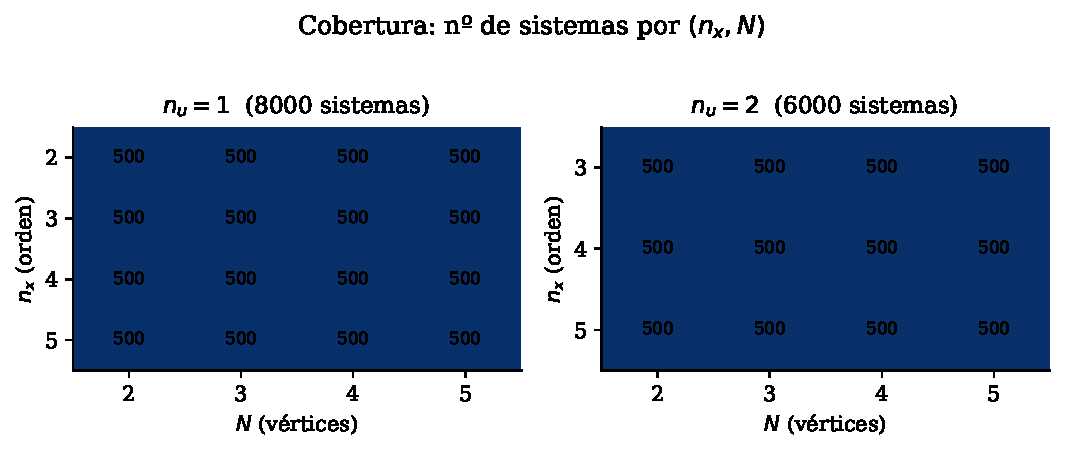
\includegraphics[width=\linewidth]{fig1_cobertura.pdf}
  \caption{Cobertura factorial: número de sistemas por $(n_x,N)$, separado por
  número de actuadores $n_u$. El soporte está completamente balanceado a $500$
  sistemas por celda.}
  \label{fig:cobertura}
\end{figure}

% --------------------------------------------------------------------
\subsection{La planta sin control (lazo abierto)}
\label{sec:db-ol}
% --------------------------------------------------------------------

``Lazo abierto'' se refiere al sistema \emph{sin} controlador. Las plantas de la
base son \emph{difíciles}: el $\mathbf{98.8\%}$ es inestable en lazo abierto
(al menos un vértice tiene un autovalor con parte real positiva), y sólo el
$1.2\%$ sería estable por sí solo. La abscisa espectral del peor vértice
(la rapidez del modo más inestable, ver Sec.~\ref{sec:db-conceptos}) tiene
mediana $30.9$ y llega hasta $\sim\!832$ (Fig.~\ref{fig:estabilidad}). En otras
palabras, la base no contiene casos triviales: el controlador debe
\emph{crear} la estabilidad, no sólo conservarla.

\begin{figure}[t]
  \centering
  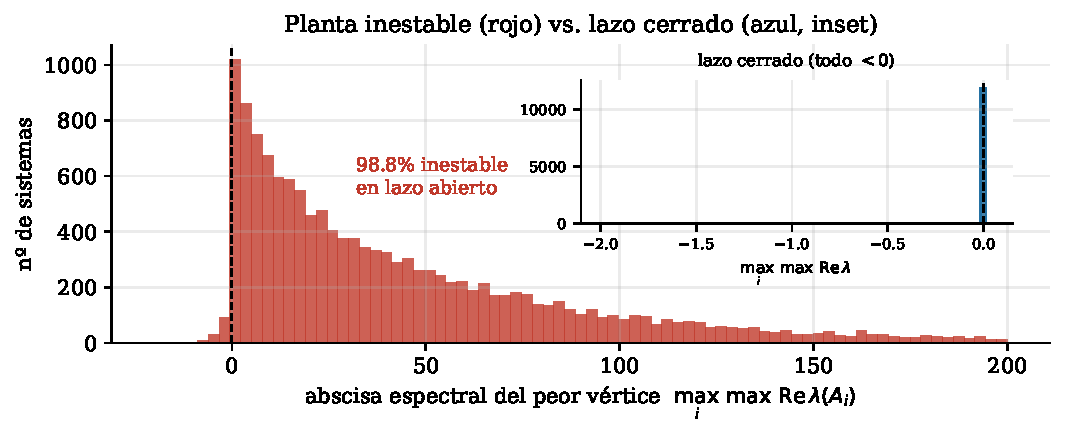
\includegraphics[width=\linewidth]{fig2_estabilidad.pdf}
  \caption{Abscisa espectral del peor vértice. Sin control la planta es
  inestable (rojo, parte real $>0$) en el $98.8\%$ de los casos; con la ganancia
  $K$ el lazo cerrado es estable en el $100\%$ (inset azul, todos $<0$).}
  \label{fig:estabilidad}
\end{figure}

En cuanto al ``tamaño'' de la dinámica (Fig.~\ref{fig:normas}), los descriptores
tienen un rango muy amplio: $\max_i\lVert A_i\rVert_2$ va de $12$ a $1012$
(mediana $131$) y crece de forma marcada con el orden $n_x$, mientras que
$\max_i\lVert B_i\rVert_2$ se mantiene acotado en $[0.74,\,16.8]$. Esta
disparidad de escalas —tres órdenes de magnitud en $\lVert A\rVert$— es
justamente la que obliga a \emph{normalizar} los datos antes de entrenar: cada
politopo se reescala dividiéndolo por su entrada de mayor magnitud,
$\gamma=\max(\max|A|,\max|B|)$, de modo que todas las cifras queden en
$[-1,1]$ y los sistemas sean comparables entre sí (esta reescala no cambia el
signo de los autovalores —y por tanto no afecta la estabilidad— aunque sí divide
la tasa de decaimiento por $\gamma$).

\begin{figure}[t]
  \centering
  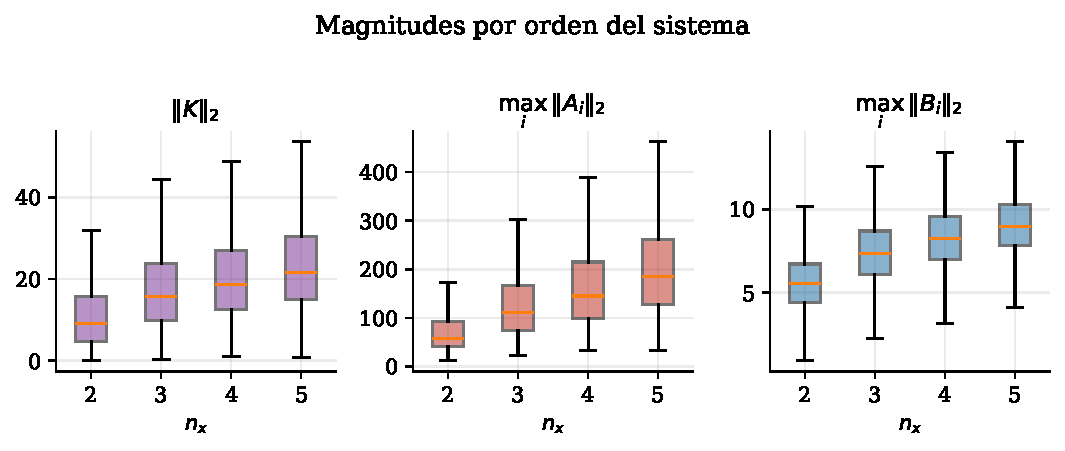
\includegraphics[width=\linewidth]{fig5_normas.pdf}
  \caption{Distribución del esfuerzo de control $\lVert K\rVert_2$ y de los
  tamaños $\max_i\lVert A_i\rVert_2$ y $\max_i\lVert B_i\rVert_2$, según el orden
  $n_x$. Ambos crecen con el orden del sistema.}
  \label{fig:normas}
\end{figure}

\paragraph{¿Se puede controlar? Controlabilidad y condicionamiento.}
Un requisito previo para que exista una ganancia estabilizante es que el sistema
sea \emph{controlable}: que desde la entrada se pueda influir en todas las
direcciones del estado. Esto se cumple en el $100\%$ de los vértices de todos
los sistemas. El número de condición de las matrices es benigno en general
($\kappa(A_i)$ con mediana $53$), con una cola pesada: un $0.39\%$ de los
sistemas supera $\kappa>10^4$, con casos extremos de hasta $5.7\times10^5$
(Fig.~\ref{fig:cond}); estos son los sistemas numéricamente delicados durante el
entrenamiento.

\begin{figure}[t]
  \centering
  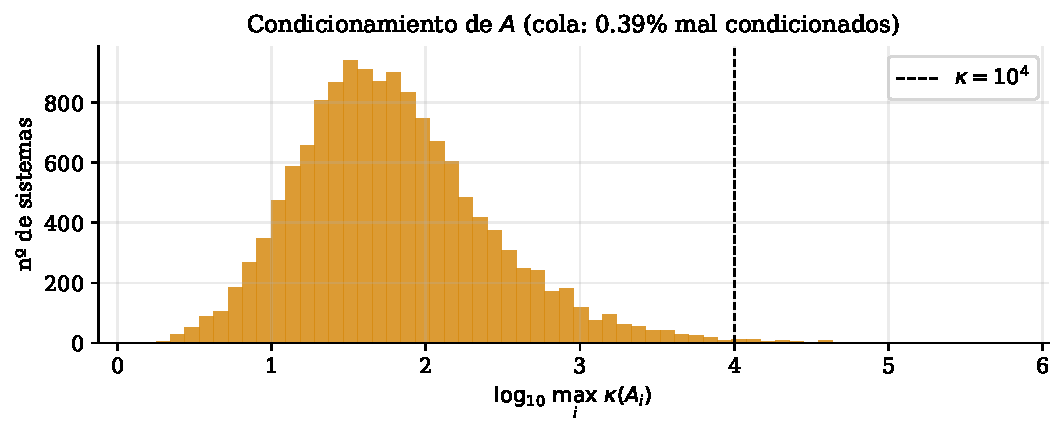
\includegraphics[width=0.82\linewidth]{fig7_condicionamiento.pdf}
  \caption{Número de condición $\max_i\kappa(A_i)$ (escala $\log_{10}$). La gran
  mayoría está bien condicionada; una cola del $0.39\%$ supera $\kappa=10^4$.}
  \label{fig:cond}
\end{figure}

% --------------------------------------------------------------------
\subsection{Tamaño de la incertidumbre (geometría del politopo)}
% --------------------------------------------------------------------

¿Qué tan ``grande'' es la incertidumbre de cada sistema? Lo medimos con la
dispersión de los vértices respecto a su promedio,
$\max_i\lVert A_i-\bar A\rVert_2$: si los vértices son muy parecidos entre sí, el
politopo es pequeño (poca incertidumbre); si son muy distintos, es grande. Su
mediana es $97.5$ y crece de forma sistemática con el número de vértices $N$
(Fig.~\ref{fig:dispersion}): más vértices implican politopos más amplios y, por
tanto, una incertidumbre más severa que la \emph{misma} ganancia $K$ debe cubrir
a la vez. Esto convierte a $N$ en un eje natural de dificultad y motiva evaluar
el modelo \emph{separado por $N$}.

\begin{figure}[t]
  \centering
  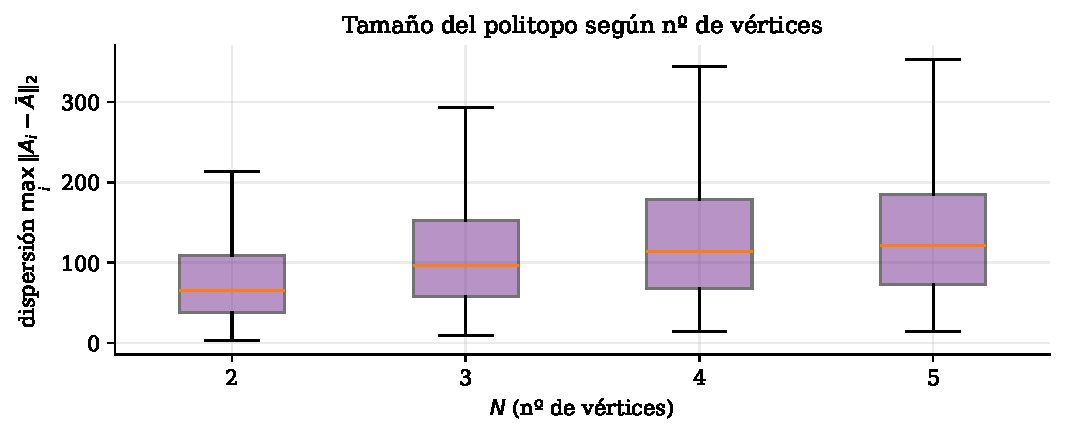
\includegraphics[width=0.82\linewidth]{fig6_dispersion.pdf}
  \caption{Tamaño del politopo $\max_i\lVert A_i-\bar A\rVert_2$ frente al número
  de vértices $N$. La incertidumbre crece con $N$.}
  \label{fig:dispersion}
\end{figure}

% --------------------------------------------------------------------
\subsection{El controlador y el sistema en lazo cerrado}
\label{sec:db-control}
% --------------------------------------------------------------------

``Lazo cerrado'' es el sistema \emph{con} el controlador conectado, gobernado por
$A_i+B_iK$. Verificamos numéricamente la etiqueta de la base recomputando los
autovalores de todos los vértices con su ganancia. El resultado es categórico:
\textbf{el $100\%$ de los $14\,000$ sistemas queda estable} (todos los
autovalores de todos los vértices con parte real negativa). No hay sistemas mal
etiquetados ni ganancias inconsistentes.

\paragraph{Estabilización ``al borde''.}
Lo más informativo es \emph{cómo} se estabiliza. La tasa de decaimiento lograda
$\alpha$ (Sec.~\ref{sec:db-conceptos}) —cuánto margen de estabilidad consigue el
controlador— se concentra masivamente junto a cero: su mediana es
$\alpha\approx 6.3\times10^{-4}$ y el $\mathbf{84.9\%}$ de los sistemas queda
\emph{casi marginal} ($\alpha<10^{-2}$), con sólo una minoría que alcanza
márgenes amplios ($\alpha_{95}=1.51$, máximo $10.6$). La distribución es
claramente \emph{bimodal} (Fig.~\ref{fig:decay}). Es decir, la ganancia de
referencia \emph{apenas} estabiliza: deja el modo dominante prácticamente sobre
la frontera de la inestabilidad.

\begin{figure}[t]
  \centering
  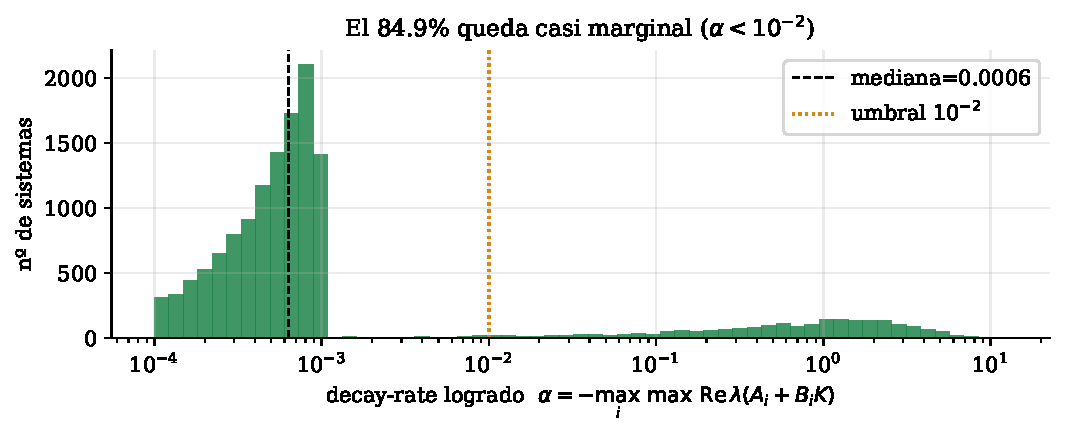
\includegraphics[width=\linewidth]{fig3_decay.pdf}
  \caption{Tasa de decaimiento lograda $\alpha$ (escala logarítmica). El
  $84.9\%$ de los sistemas queda casi marginal ($\alpha<10^{-2}$); una minoría
  exhibe márgenes grandes. La distribución es bimodal.}
  \label{fig:decay}
\end{figure}

Este comportamiento sugiere que las ganancias se construyeron buscando
\emph{cualquier} solución válida (factibilidad), no la más rápida. Lo respalda
un detalle: aunque el modo \emph{dominante} se aparca en la frontera, el resto de
los modos se empujan muy hacia la zona estable —la mediana de la parte real
sobre \emph{todos} los autovalores de lazo cerrado es $-21.4$. Visualmente, el
controlador ``refleja'' el espectro de la planta desde el semiplano inestable
(derecho) al estable (izquierdo), dejando un único modo lento que fija $\alpha$
(Fig.~\ref{fig:plano}).

\begin{figure}[t]
  \centering
  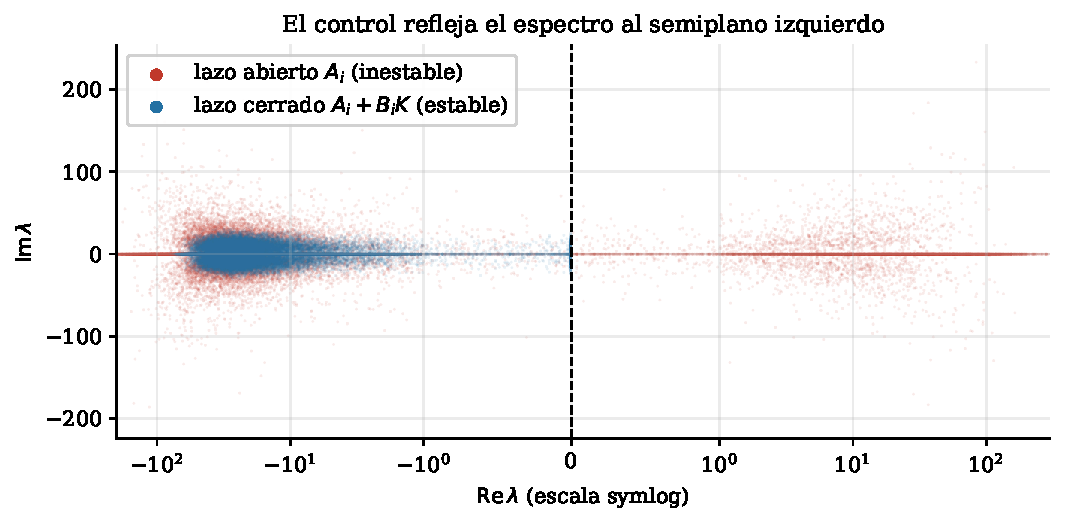
\includegraphics[width=\linewidth]{fig4_plano_complejo.pdf}
  \caption{Autovalores de los vértices en el plano complejo (eje horizontal en
  escala symlog). Sin control (rojo) la planta tiene autovalores en el semiplano
  derecho (inestables); con control (azul) todos pasan al semiplano izquierdo
  (estables), con el modo dominante pegado al eje.}
  \label{fig:plano}
\end{figure}

\paragraph{Esfuerzo de control.}
Lo ``caro'' que resulta controlar cada sistema se mide con $\lVert K\rVert_2$
(mediana $17.4$, máximo $98.1$). No es arbitrario: crece junto con el tamaño de
la planta ($\rho_{\text{Spearman}}=0.90$ frente a $\lVert A\rVert$), el tamaño
del politopo ($0.85$ frente a la dispersión) y la inestabilidad de lazo abierto
($0.63$); plantas más grandes e inestables exigen controladores más fuertes
(Fig.~\ref{fig:corr}). En cambio, la tasa de decaimiento $\alpha$ es
\emph{estadísticamente independiente} de todos los descriptores ($|\rho|\le0.04$
en todos los casos): el margen marginal no se debe a que el problema sea difícil,
sino a la forma en que se construyó la ganancia.

\begin{figure}[t]
  \centering
  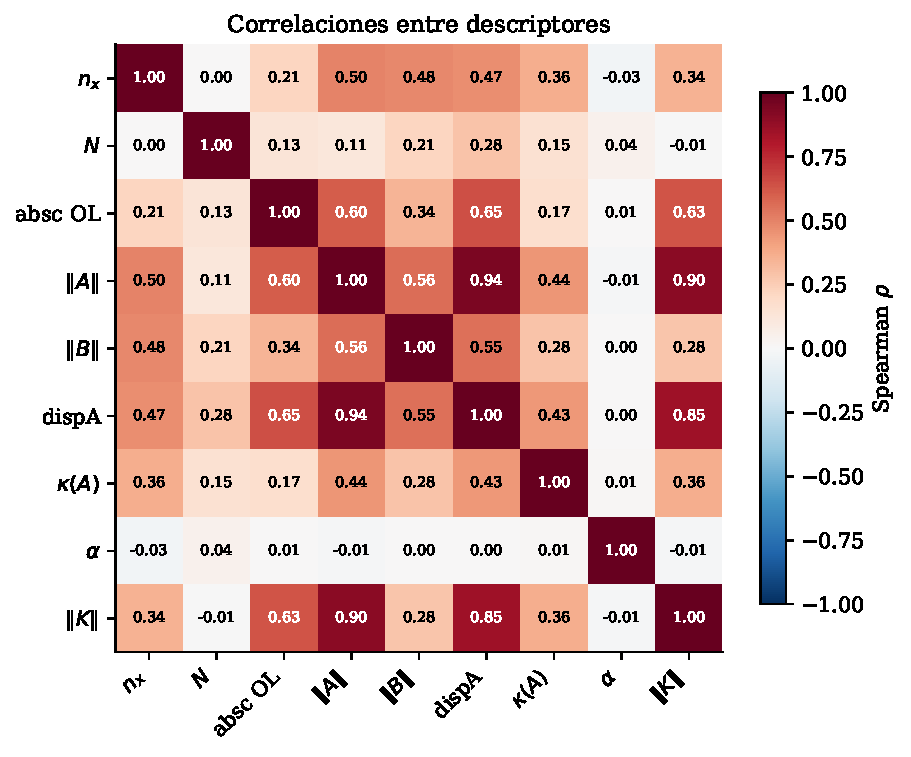
\includegraphics[width=0.78\linewidth]{fig8_correlaciones.pdf}
  \caption{Correlaciones de rango (Spearman) entre indicadores. El esfuerzo
  $\lVert K\rVert$ sigue al tamaño de la planta y del politopo; la tasa de
  decaimiento $\alpha$ no correlaciona con ningún indicador.}
  \label{fig:corr}
\end{figure}

% --------------------------------------------------------------------
\subsection{Calidad de los datos}
% --------------------------------------------------------------------

\begin{itemize}
  \item \textbf{Completitud:} sin valores faltantes en el soporte; las $28$
        celdas válidas están pobladas a $500/500$.
  \item \textbf{Validez de la etiqueta:} $100\%$ de los sistemas verificados como
        efectivamente estabilizados por su $K$ (todos los vértices estables).
  \item \textbf{Controlabilidad:} $100\%$ de los vértices controlables.
  \item \textbf{Duplicados:} no se detectaron sistemas repetidos.
  \item \textbf{Valores atípicos:} acotados y plausibles; la única cola de
        cuidado es el condicionamiento numérico ($0.39\%$ con $\kappa>10^4$),
        relevante para la estabilidad del cálculo más que para la validez del dato.
\end{itemize}

\begin{table}[t]
  \centering
  \caption{Resumen de indicadores sobre los $14\,000$ sistemas (datos crudos,
  sin normalizar).}
  \label{tab:resumen}
  \begin{tabular}{lrrr}
    \toprule
    Indicador & Mín. & Mediana & Máx. \\
    \midrule
    Abscisa espectral peor vértice (sin control) & $-17.9$ & $30.9$ & $832$ \\
    Tasa de decaimiento lograda $\alpha$         & $1.0\times10^{-4}$ & $6.3\times10^{-4}$ & $10.6$ \\
    $\max_i\lVert A_i\rVert_2$ (tamaño de la dinámica) & $12.2$ & $131$ & $1012$ \\
    $\max_i\lVert B_i\rVert_2$ (autoridad del control) & $0.74$ & $7.90$ & $16.8$ \\
    Dispersión del politopo (incertidumbre)      & $3.12$ & $97.5$ & $850$ \\
    Condición $\max_i\kappa(A_i)$                 & $1.44$ & $52.8$ & $5.7\times10^{5}$ \\
    Esfuerzo de control $\lVert K\rVert_2$        & $0.077$ & $17.4$ & $98.1$ \\
    \bottomrule
  \end{tabular}
\end{table}

% --------------------------------------------------------------------
\subsection{Implicaciones para el aprendizaje}
% --------------------------------------------------------------------

El análisis orienta varias decisiones de modelado:
%
\begin{enumerate}
  \item \textbf{Normalización imprescindible.} El rango de tamaños de $\lVert
        A\rVert$ (tres órdenes de magnitud) hace inviable alimentar las matrices
        crudas a la red; la reescala por $\gamma$ es necesaria para que el
        aprendizaje esté bien condicionado.
  \item \textbf{Invarianzas a aprovechar.} Un sistema es un \emph{conjunto} de
        vértices $\{(A_i,B_i)\}$ cuyo orden no importa y cuya cantidad $N$ varía,
        pero el certificado $K$ es común; esto motiva un codificador invariante
        al orden y a la cantidad de vértices (y, análogamente, al número de
        actuadores $n_u$).
  \item \textbf{Evaluar separado por $N$.} Como la incertidumbre crece con el
        número de vértices, conviene reportar el desempeño desglosado por $N$.
  \item \textbf{Sobre la señal de entrenamiento.} La ganancia de referencia es
        casi marginal y su $\alpha$ no aporta información sobre el sistema; esto
        respalda usar un objetivo \emph{auto-supervisado} —estabilizar con un
        margen $\alpha$ prescrito— en lugar de copiar directamente la $K$
        almacenada.
\end{enumerate}

%  Requiere: graphicx, booktabs, amsmath, amssymb
%  \graphicspath{{figuras/}}  % o ajusta la ruta a tus figuras
% =====================================================================

\section{Caracterización de la base de datos}
\label{sec:analisis-db}

% --------------------------------------------------------------------
\subsection{Propósito y estructura}
% --------------------------------------------------------------------

La base de datos \texttt{DB\_ssf\_RS\_500\_c.mat} es el conjunto de
entrenamiento del modelo. Cada muestra describe un \emph{sistema dinámico
incierto} junto con un controlador que lo estabiliza. Conviene fijar primero la
intuición de qué es cada cosa antes de cuantificarla.

Un \textbf{sistema lineal} modela cómo evoluciona en el tiempo un vector de
estado $x(t)\in\mathbb{R}^{n_x}$ (las variables internas del proceso) cuando se
le aplica una señal de control $u(t)\in\mathbb{R}^{n_u}$:
%
\begin{equation}
  \dot{x}(t) = A\,x(t) + B\,u(t).
  \label{eq:lti}
\end{equation}
%
La matriz $A$ codifica la \emph{dinámica propia} del sistema (cómo se influyen
entre sí las variables si no hiciéramos nada), y $B$ describe \emph{cómo entra
el control} en esa dinámica. El número $n_x$ es el \emph{orden} (cuántas
variables de estado) y $n_u$ es el número de \emph{actuadores} (cuántas
perillas de control independientes hay).

En la práctica el sistema no se conoce con exactitud: hay incertidumbre en sus
parámetros. Se modela esa incertidumbre con un \textbf{politopo}, es decir, una
familia de sistemas posibles obtenida ``mezclando'' $N$ casos extremos
conocidos —los \emph{vértices} $(A_i,B_i)$— en todas las proporciones
convexas:
%
\begin{equation}
  \bigl(A(\theta),B(\theta)\bigr)=\sum_{i=1}^{N}\theta_i\,(A_i,B_i),
  \qquad \theta_i\ge 0,\ \textstyle\sum_i\theta_i=1.
  \label{eq:politopo}
\end{equation}
%
Intuitivamente, el sistema real es \emph{algún} punto dentro de la envolvente
convexa de esos $N$ vértices, pero no sabemos cuál; un controlador
\emph{robusto} debe funcionar para todos a la vez. Esto es análogo, en
términos de computación, a exigir una garantía en el \emph{peor caso} sobre un
conjunto acotado de entradas posibles.

Cada muestra de la base es por tanto una terna: el conjunto de vértices
$\{A_i\}$, el conjunto $\{B_i\}$, y una \textbf{ganancia} $K\in\mathbb{R}^{n_u\times
n_x}$ que define el controlador por realimentación de estado $u(t)=K\,x(t)$ —una
única $K$ que estabiliza todo el politopo (Tabla~\ref{tab:esquema}). La etiqueta
\texttt{RS} (\emph{robustly stabilizable}) indica que el sistema admite tal
ganancia robusta.\footnote{\textbf{Procedencia (por confirmar con el autor de la
base):} la evidencia empírica (Sec.~\ref{sec:db-control}) es consistente con que
cada $K$ se obtuvo resolviendo un problema de factibilidad (una LMI de
estabilizabilidad cuadrática), sin optimizar la rapidez de la respuesta. Falta
confirmar cómo se generaron los vértices $(A_i,B_i)$.}

\begin{table}[t]
  \centering
  \caption{Esquema de la base de datos. Cada sistema es un politopo de $N$
  vértices con una ganancia robusta $K$.}
  \label{tab:esquema}
  \begin{tabular}{llll}
    \toprule
    Campo & Símbolo & Forma & Descripción \\
    \midrule
    \texttt{A} & $\{A_i\}_{i=1}^N$ & $N\times(n_x\!\times\! n_x)$ & Dinámica propia de cada vértice \\
    \texttt{B} & $\{B_i\}_{i=1}^N$ & $N\times(n_x\!\times\! n_u)$ & Entrada de control de cada vértice \\
    \texttt{K} & $K$               & $n_u\times n_x$             & Ganancia del controlador (común) \\
    \midrule
    \multicolumn{4}{l}{$n_x\in\{2,3,4,5\}$\quad $n_u\in\{1,2\}$\quad $N\in\{2,3,4,5\}$\quad $500$ casos/celda} \\
    \bottomrule
  \end{tabular}
\end{table}

% --------------------------------------------------------------------
\subsection{Cómo se mide un sistema y su estabilidad}
\label{sec:db-conceptos}
% --------------------------------------------------------------------

Para caracterizar la base usamos un puñado de indicadores numéricos. Como el
lector no tiene por qué venir de teoría de control, los explicamos aquí en
lenguaje llano; la Tabla~\ref{tab:glosario} los resume.

\paragraph{Estabilidad y autovalores.}
La pregunta central sobre un sistema es si es \emph{estable}: si lo perturbamos,
¿vuelve al equilibrio o se dispara? Para un sistema lineal
$\dot{x}=Ax$, la respuesta la dan los \textbf{autovalores} de $A$. Toda
solución es una combinación de ``modos'' de la forma $e^{\lambda t}$, donde
$\lambda=a+bi$ es un autovalor. Su \emph{parte real} $a=\operatorname{Re}\lambda$
controla la magnitud ($e^{at}$ crece si $a>0$ y decae si $a<0$) y su parte
imaginaria $b$ controla la oscilación. Por tanto:
%
\begin{center}
  \emph{el sistema es estable} $\iff$ \emph{todos} sus autovalores cumplen
  $\operatorname{Re}\lambda<0$.
\end{center}
%
En el plano complejo, esto es ``todos los autovalores en el semiplano
izquierdo''.

\paragraph{Abscisa espectral: el modo que decide.}
No hace falta mirar todos los autovalores: basta el \emph{peor}. La
\textbf{abscisa espectral} es el mayor de las partes reales,
$\max\operatorname{Re}\lambda(A)$. Es el modo que crece más rápido (o decae más
lento) y, por sí solo, decide la estabilidad: si la abscisa es negativa, todos
los modos decaen; si es positiva, al menos uno explota. Un valor de, por
ejemplo, $832$ significa que el modo dominante crece como $e^{832\,t}$: una
inestabilidad extremadamente violenta. Lo usamos como \emph{medida relativa de
qué tan inestable} es una planta (no tiene unidades físicas porque los sistemas
son sintéticos).

\paragraph{Los dos ``máximos''.}
En las fórmulas aparecen \emph{dos} máximos anidados, y conviene separarlos:
%
\begin{equation*}
  \underbrace{\max_{i=1,\dots,N}}_{\text{(2) peor \emph{vértice}}}
  \ \underbrace{\max\,\operatorname{Re}\,\lambda(A_i)}_{\text{(1) peor \emph{modo} de ese vértice}}.
\end{equation*}
%
El máximo interno (1) recorre los autovalores de \emph{un} vértice y se queda
con su modo dominante (la abscisa espectral de $A_i$). El máximo externo (2)
recorre los $N$ vértices del politopo y se queda con el más desfavorable. La
combinación es la lectura de \emph{peor caso}: ``de toda la familia de sistemas
posibles, ¿qué tan mal se comporta el peor de ellos?''.

\paragraph{Norma de una matriz: su ``tamaño''.}
La norma espectral $\lVert A\rVert_2$ mide cuánto puede \emph{amplificar} esa
matriz a un vector (formalmente, su mayor valor singular). Es una medida del
``tamaño'' o la fuerza de la dinámica: una $\lVert A\rVert_2$ grande indica
acoplamientos internos intensos. Reportamos $\max_i\lVert A_i\rVert_2$, el
tamaño del vértice más grande del politopo.

\paragraph{Tasa de decaimiento $\alpha$: el margen de seguridad.}
Una vez cerrado el lazo con el controlador, la matriz que gobierna la dinámica
pasa a ser $A_i+B_iK$. Su abscisa espectral, cambiada de signo, es la
\textbf{tasa de decaimiento}
$\alpha=-\max_i\max\operatorname{Re}\lambda(A_i+B_iK)$. Mide \emph{qué tan
rápido} se extingue la peor respuesta: $\alpha>0$ garantiza estabilidad, y
cuanto mayor sea $\alpha$, más rápido y con más margen vuelve el sistema al
equilibrio. Un $\alpha\approx0$ significa ``estable, pero al borde'': el sistema
apenas se sostiene sobre la frontera de la inestabilidad.

\paragraph{Otros indicadores.}
La \emph{dispersión del politopo} $\max_i\lVert A_i-\bar A\rVert_2$ (con $\bar A$
el promedio de los vértices) mide qué tan distintos son los vértices entre sí,
es decir, cuánta incertidumbre hay. El \emph{número de condición} $\kappa(A_i)$
mide la sensibilidad numérica de la matriz (valores altos anticipan problemas de
precisión). El \emph{esfuerzo de control} $\lVert K\rVert_2$ mide qué tan
``agresivo'' es el controlador.

\begin{table}[t]
  \centering
  \caption{Glosario de indicadores usados en el análisis.}
  \label{tab:glosario}
  \small
  \begin{tabular}{p{3.0cm}p{3.4cm}p{6.6cm}}
    \toprule
    Indicador & En palabras simples & Un valor alto significa\dots \\
    \midrule
    Abscisa espectral (lazo abierto)\newline $\max_i\max\operatorname{Re}\lambda(A_i)$
      & Rapidez del modo más inestable del peor vértice
      & Planta muy inestable: sin control, se dispara muy rápido. \\
    Tasa de decaimiento\newline $\alpha=-\max_i\max\operatorname{Re}\lambda(A_i+B_iK)$
      & Qué tan rápido se calma el sistema ya controlado
      & Más margen de estabilidad; $\alpha\approx0$ = estable al borde. \\
    Norma $\max_i\lVert A_i\rVert_2$
      & ``Tamaño''/fuerza de la dinámica propia
      & Acoplamientos internos intensos. \\
    Norma $\max_i\lVert B_i\rVert_2$
      & Cuánto influye el control en el estado
      & Actuadores con mucha autoridad. \\
    Dispersión del politopo\newline $\max_i\lVert A_i-\bar A\rVert_2$
      & Qué tan distintos son los vértices
      & Más incertidumbre que cubrir con una sola $K$. \\
    Condición $\kappa(A_i)$
      & Sensibilidad numérica de la matriz
      & Riesgo de imprecisión numérica. \\
    Esfuerzo $\lVert K\rVert_2$
      & Qué tan ``fuerte'' es el controlador
      & Acción de control más agresiva. \\
    \bottomrule
  \end{tabular}
\end{table}

% --------------------------------------------------------------------
\subsection{Cobertura y diseño experimental}
% --------------------------------------------------------------------

El archivo organiza las muestras en un arreglo de cuatro índices,
$\texttt{BASE}[\,n_x,\,n_u,\,N,\,\text{caso}\,]$, de forma nominal
$5\times 2\times 5\times 500$. La malla está poblada parcialmente: el orden
mínimo depende del número de actuadores ($n_u{=}1\Rightarrow n_x\in\{2,\dots,5\}$;
$n_u{=}2\Rightarrow n_x\in\{3,4,5\}$) y siempre $N\ge 2$. De las $25\,000$
posiciones nominales sólo $28$ están ocupadas, con exactamente $500$ casos cada
una: en total $\mathbf{14\,000}$ sistemas ($8\,000$ con $n_u{=}1$ y $6\,000$ con
$n_u{=}2$).

La base sigue así un \emph{diseño factorial completo y perfectamente
balanceado} sobre los factores $(n_x, n_u, N)$ admisibles
(Fig.~\ref{fig:cobertura}): las $28$ combinaciones válidas aparecen con la misma
cantidad de ejemplos ($500$), sin celdas faltantes ni sobre-representadas. Este
balance es deseable para el aprendizaje: evita que el modelo privilegie una
configuración por mero desbalance de frecuencia, y permite reportar métricas
separadas por $N$ y por $n_x$ sin correcciones.

\begin{figure}[t]
  \centering
  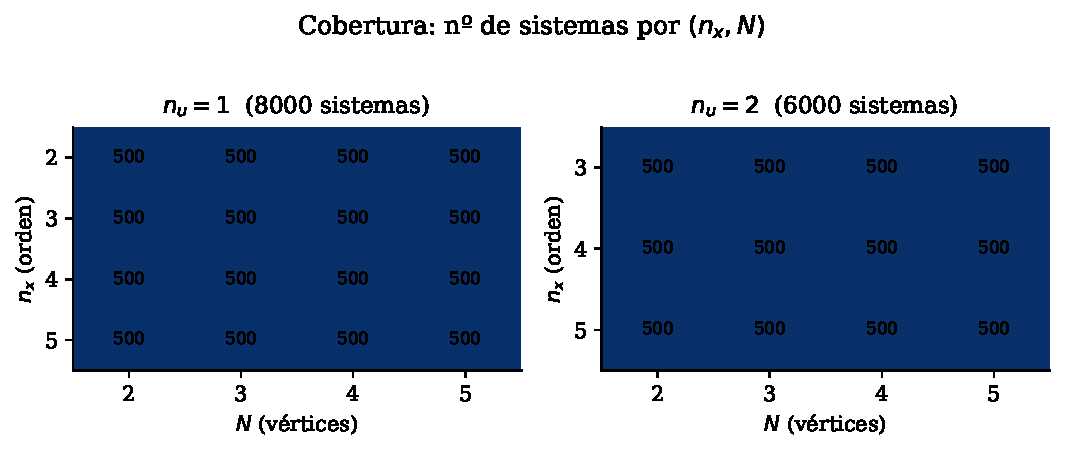
\includegraphics[width=\linewidth]{fig1_cobertura.pdf}
  \caption{Cobertura factorial: número de sistemas por $(n_x,N)$, separado por
  número de actuadores $n_u$. El soporte está completamente balanceado a $500$
  sistemas por celda.}
  \label{fig:cobertura}
\end{figure}

% --------------------------------------------------------------------
\subsection{La planta sin control (lazo abierto)}
\label{sec:db-ol}
% --------------------------------------------------------------------

``Lazo abierto'' se refiere al sistema \emph{sin} controlador. Las plantas de la
base son \emph{difíciles}: el $\mathbf{98.8\%}$ es inestable en lazo abierto
(al menos un vértice tiene un autovalor con parte real positiva), y sólo el
$1.2\%$ sería estable por sí solo. La abscisa espectral del peor vértice
(la rapidez del modo más inestable, ver Sec.~\ref{sec:db-conceptos}) tiene
mediana $30.9$ y llega hasta $\sim\!832$ (Fig.~\ref{fig:estabilidad}). En otras
palabras, la base no contiene casos triviales: el controlador debe
\emph{crear} la estabilidad, no sólo conservarla.

\begin{figure}[t]
  \centering
  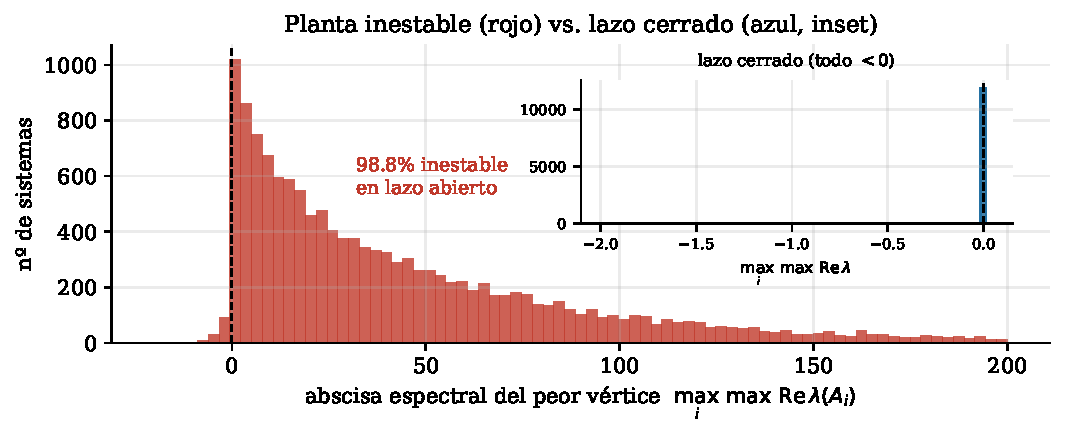
\includegraphics[width=\linewidth]{fig2_estabilidad.pdf}
  \caption{Abscisa espectral del peor vértice. Sin control la planta es
  inestable (rojo, parte real $>0$) en el $98.8\%$ de los casos; con la ganancia
  $K$ el lazo cerrado es estable en el $100\%$ (inset azul, todos $<0$).}
  \label{fig:estabilidad}
\end{figure}

En cuanto al ``tamaño'' de la dinámica (Fig.~\ref{fig:normas}), los descriptores
tienen un rango muy amplio: $\max_i\lVert A_i\rVert_2$ va de $12$ a $1012$
(mediana $131$) y crece de forma marcada con el orden $n_x$, mientras que
$\max_i\lVert B_i\rVert_2$ se mantiene acotado en $[0.74,\,16.8]$. Esta
disparidad de escalas —tres órdenes de magnitud en $\lVert A\rVert$— es
justamente la que obliga a \emph{normalizar} los datos antes de entrenar: cada
politopo se reescala dividiéndolo por su entrada de mayor magnitud,
$\gamma=\max(\max|A|,\max|B|)$, de modo que todas las cifras queden en
$[-1,1]$ y los sistemas sean comparables entre sí (esta reescala no cambia el
signo de los autovalores —y por tanto no afecta la estabilidad— aunque sí divide
la tasa de decaimiento por $\gamma$).

\begin{figure}[t]
  \centering
  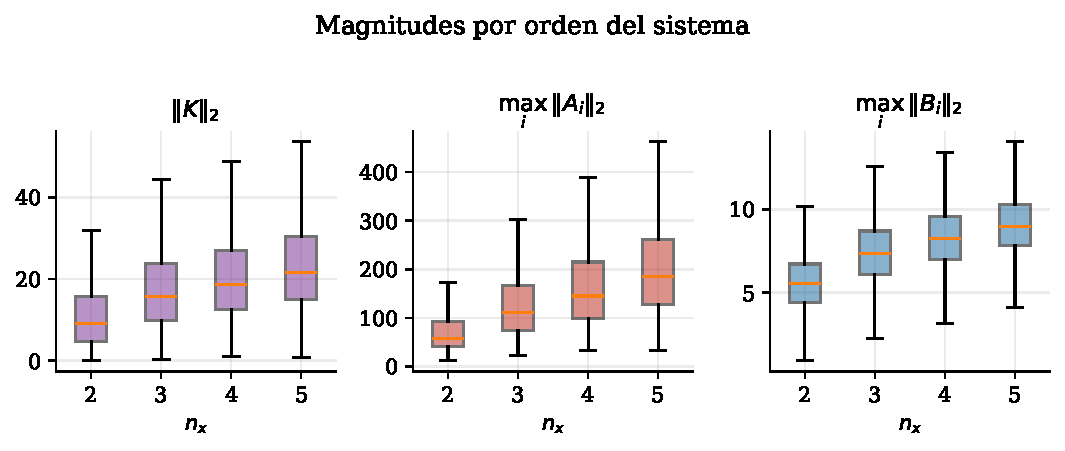
\includegraphics[width=\linewidth]{fig5_normas.pdf}
  \caption{Distribución del esfuerzo de control $\lVert K\rVert_2$ y de los
  tamaños $\max_i\lVert A_i\rVert_2$ y $\max_i\lVert B_i\rVert_2$, según el orden
  $n_x$. Ambos crecen con el orden del sistema.}
  \label{fig:normas}
\end{figure}

\paragraph{¿Se puede controlar? Controlabilidad y condicionamiento.}
Un requisito previo para que exista una ganancia estabilizante es que el sistema
sea \emph{controlable}: que desde la entrada se pueda influir en todas las
direcciones del estado. Esto se cumple en el $100\%$ de los vértices de todos
los sistemas. El número de condición de las matrices es benigno en general
($\kappa(A_i)$ con mediana $53$), con una cola pesada: un $0.39\%$ de los
sistemas supera $\kappa>10^4$, con casos extremos de hasta $5.7\times10^5$
(Fig.~\ref{fig:cond}); estos son los sistemas numéricamente delicados durante el
entrenamiento.

\begin{figure}[t]
  \centering
  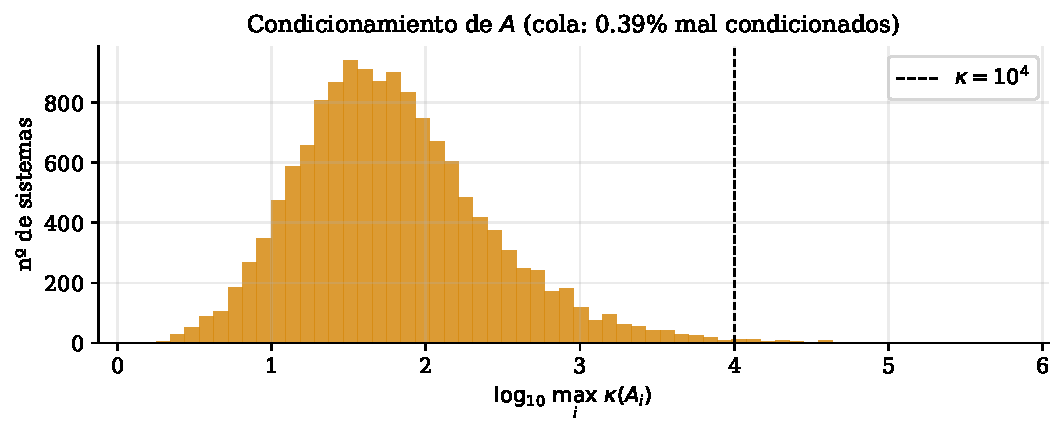
\includegraphics[width=0.82\linewidth]{fig7_condicionamiento.pdf}
  \caption{Número de condición $\max_i\kappa(A_i)$ (escala $\log_{10}$). La gran
  mayoría está bien condicionada; una cola del $0.39\%$ supera $\kappa=10^4$.}
  \label{fig:cond}
\end{figure}

% --------------------------------------------------------------------
\subsection{Tamaño de la incertidumbre (geometría del politopo)}
% --------------------------------------------------------------------

¿Qué tan ``grande'' es la incertidumbre de cada sistema? Lo medimos con la
dispersión de los vértices respecto a su promedio,
$\max_i\lVert A_i-\bar A\rVert_2$: si los vértices son muy parecidos entre sí, el
politopo es pequeño (poca incertidumbre); si son muy distintos, es grande. Su
mediana es $97.5$ y crece de forma sistemática con el número de vértices $N$
(Fig.~\ref{fig:dispersion}): más vértices implican politopos más amplios y, por
tanto, una incertidumbre más severa que la \emph{misma} ganancia $K$ debe cubrir
a la vez. Esto convierte a $N$ en un eje natural de dificultad y motiva evaluar
el modelo \emph{separado por $N$}.

\begin{figure}[t]
  \centering
  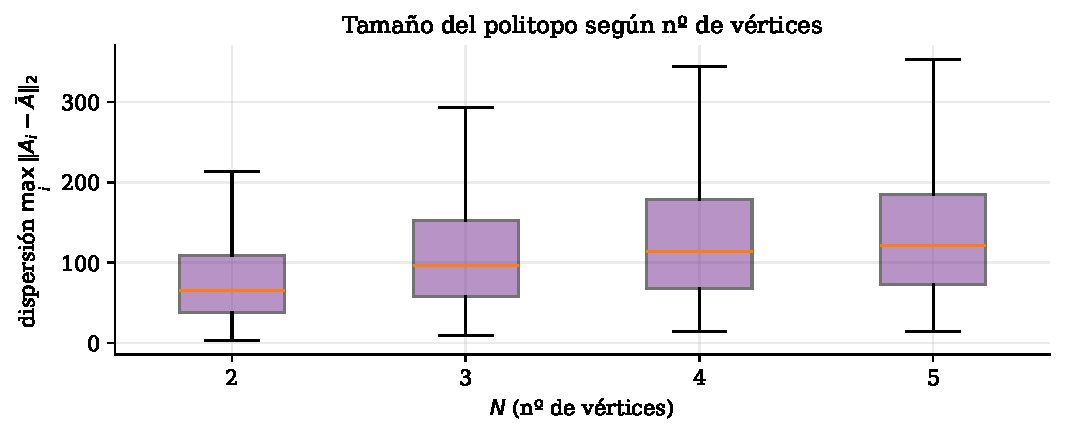
\includegraphics[width=0.82\linewidth]{fig6_dispersion.pdf}
  \caption{Tamaño del politopo $\max_i\lVert A_i-\bar A\rVert_2$ frente al número
  de vértices $N$. La incertidumbre crece con $N$.}
  \label{fig:dispersion}
\end{figure}

% --------------------------------------------------------------------
\subsection{El controlador y el sistema en lazo cerrado}
\label{sec:db-control}
% --------------------------------------------------------------------

``Lazo cerrado'' es el sistema \emph{con} el controlador conectado, gobernado por
$A_i+B_iK$. Verificamos numéricamente la etiqueta de la base recomputando los
autovalores de todos los vértices con su ganancia. El resultado es categórico:
\textbf{el $100\%$ de los $14\,000$ sistemas queda estable} (todos los
autovalores de todos los vértices con parte real negativa). No hay sistemas mal
etiquetados ni ganancias inconsistentes.

\paragraph{Estabilización ``al borde''.}
Lo más informativo es \emph{cómo} se estabiliza. La tasa de decaimiento lograda
$\alpha$ (Sec.~\ref{sec:db-conceptos}) —cuánto margen de estabilidad consigue el
controlador— se concentra masivamente junto a cero: su mediana es
$\alpha\approx 6.3\times10^{-4}$ y el $\mathbf{84.9\%}$ de los sistemas queda
\emph{casi marginal} ($\alpha<10^{-2}$), con sólo una minoría que alcanza
márgenes amplios ($\alpha_{95}=1.51$, máximo $10.6$). La distribución es
claramente \emph{bimodal} (Fig.~\ref{fig:decay}). Es decir, la ganancia de
referencia \emph{apenas} estabiliza: deja el modo dominante prácticamente sobre
la frontera de la inestabilidad.

\begin{figure}[t]
  \centering
  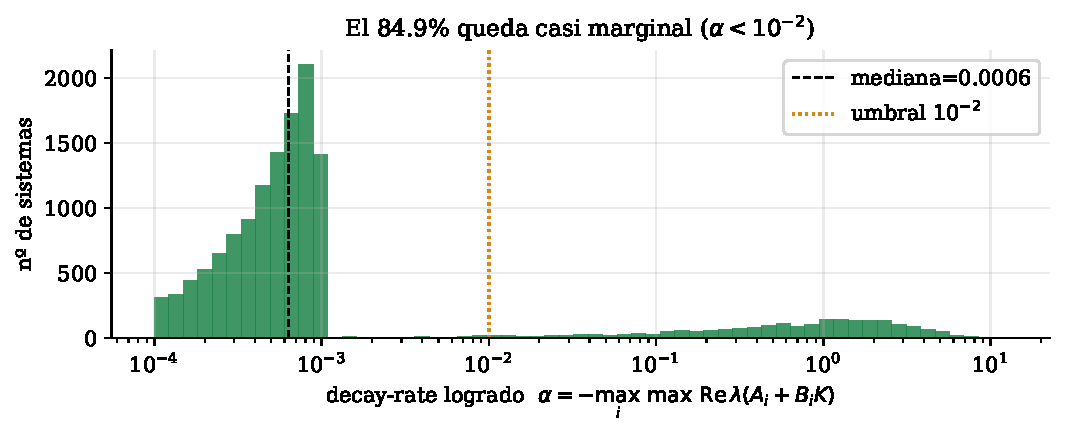
\includegraphics[width=\linewidth]{fig3_decay.pdf}
  \caption{Tasa de decaimiento lograda $\alpha$ (escala logarítmica). El
  $84.9\%$ de los sistemas queda casi marginal ($\alpha<10^{-2}$); una minoría
  exhibe márgenes grandes. La distribución es bimodal.}
  \label{fig:decay}
\end{figure}

Este comportamiento sugiere que las ganancias se construyeron buscando
\emph{cualquier} solución válida (factibilidad), no la más rápida. Lo respalda
un detalle: aunque el modo \emph{dominante} se aparca en la frontera, el resto de
los modos se empujan muy hacia la zona estable —la mediana de la parte real
sobre \emph{todos} los autovalores de lazo cerrado es $-21.4$. Visualmente, el
controlador ``refleja'' el espectro de la planta desde el semiplano inestable
(derecho) al estable (izquierdo), dejando un único modo lento que fija $\alpha$
(Fig.~\ref{fig:plano}).

\begin{figure}[t]
  \centering
  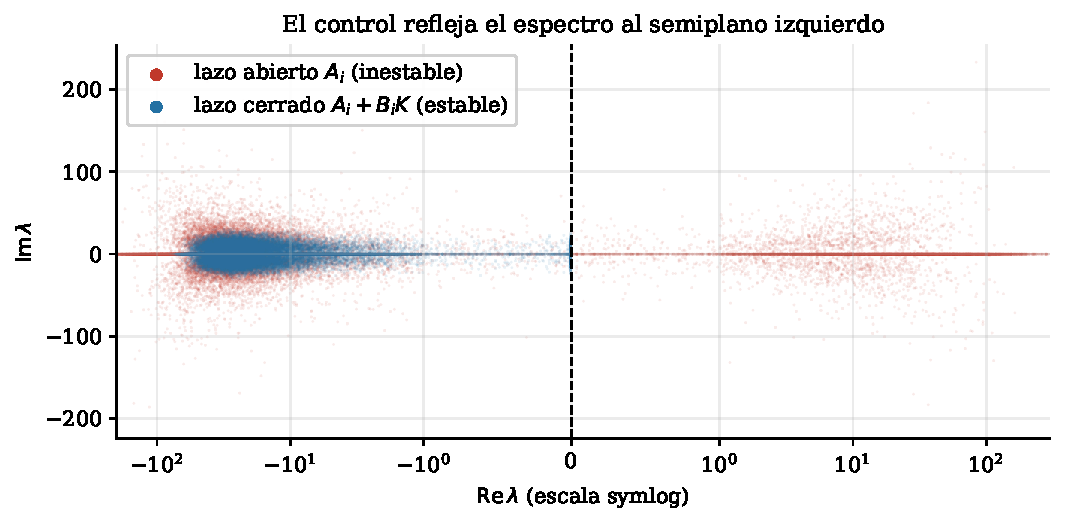
\includegraphics[width=\linewidth]{fig4_plano_complejo.pdf}
  \caption{Autovalores de los vértices en el plano complejo (eje horizontal en
  escala symlog). Sin control (rojo) la planta tiene autovalores en el semiplano
  derecho (inestables); con control (azul) todos pasan al semiplano izquierdo
  (estables), con el modo dominante pegado al eje.}
  \label{fig:plano}
\end{figure}

\paragraph{Esfuerzo de control.}
Lo ``caro'' que resulta controlar cada sistema se mide con $\lVert K\rVert_2$
(mediana $17.4$, máximo $98.1$). No es arbitrario: crece junto con el tamaño de
la planta ($\rho_{\text{Spearman}}=0.90$ frente a $\lVert A\rVert$), el tamaño
del politopo ($0.85$ frente a la dispersión) y la inestabilidad de lazo abierto
($0.63$); plantas más grandes e inestables exigen controladores más fuertes
(Fig.~\ref{fig:corr}). En cambio, la tasa de decaimiento $\alpha$ es
\emph{estadísticamente independiente} de todos los descriptores ($|\rho|\le0.04$
en todos los casos): el margen marginal no se debe a que el problema sea difícil,
sino a la forma en que se construyó la ganancia.

\begin{figure}[t]
  \centering
  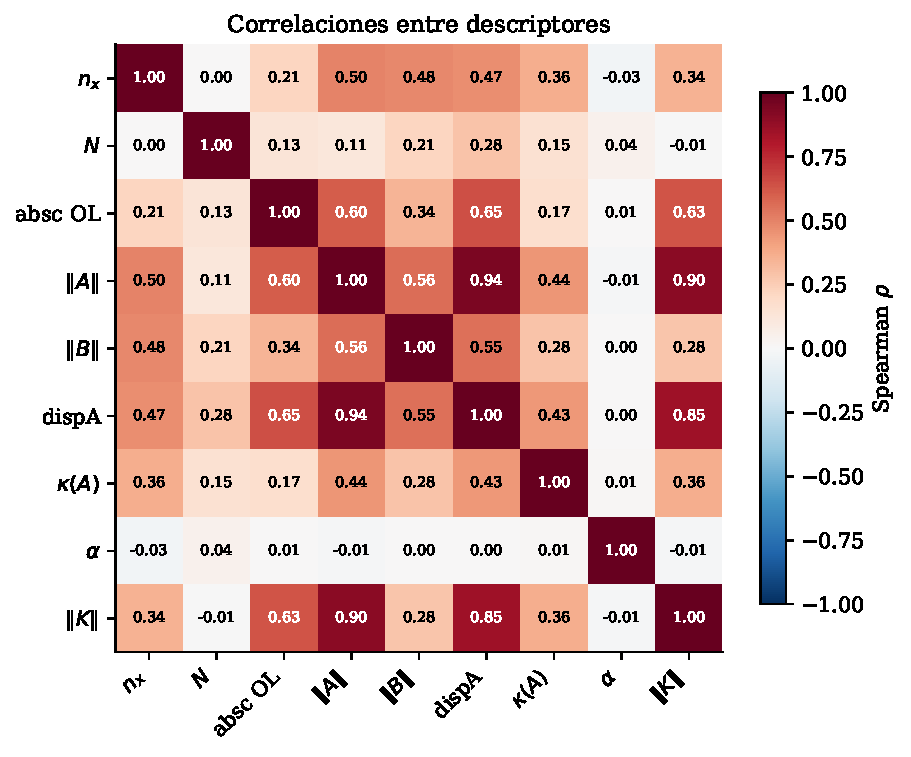
\includegraphics[width=0.78\linewidth]{fig8_correlaciones.pdf}
  \caption{Correlaciones de rango (Spearman) entre indicadores. El esfuerzo
  $\lVert K\rVert$ sigue al tamaño de la planta y del politopo; la tasa de
  decaimiento $\alpha$ no correlaciona con ningún indicador.}
  \label{fig:corr}
\end{figure}

% --------------------------------------------------------------------
\subsection{Calidad de los datos}
% --------------------------------------------------------------------

\begin{itemize}
  \item \textbf{Completitud:} sin valores faltantes en el soporte; las $28$
        celdas válidas están pobladas a $500/500$.
  \item \textbf{Validez de la etiqueta:} $100\%$ de los sistemas verificados como
        efectivamente estabilizados por su $K$ (todos los vértices estables).
  \item \textbf{Controlabilidad:} $100\%$ de los vértices controlables.
  \item \textbf{Duplicados:} no se detectaron sistemas repetidos.
  \item \textbf{Valores atípicos:} acotados y plausibles; la única cola de
        cuidado es el condicionamiento numérico ($0.39\%$ con $\kappa>10^4$),
        relevante para la estabilidad del cálculo más que para la validez del dato.
\end{itemize}

\begin{table}[t]
  \centering
  \caption{Resumen de indicadores sobre los $14\,000$ sistemas (datos crudos,
  sin normalizar).}
  \label{tab:resumen}
  \begin{tabular}{lrrr}
    \toprule
    Indicador & Mín. & Mediana & Máx. \\
    \midrule
    Abscisa espectral peor vértice (sin control) & $-17.9$ & $30.9$ & $832$ \\
    Tasa de decaimiento lograda $\alpha$         & $1.0\times10^{-4}$ & $6.3\times10^{-4}$ & $10.6$ \\
    $\max_i\lVert A_i\rVert_2$ (tamaño de la dinámica) & $12.2$ & $131$ & $1012$ \\
    $\max_i\lVert B_i\rVert_2$ (autoridad del control) & $0.74$ & $7.90$ & $16.8$ \\
    Dispersión del politopo (incertidumbre)      & $3.12$ & $97.5$ & $850$ \\
    Condición $\max_i\kappa(A_i)$                 & $1.44$ & $52.8$ & $5.7\times10^{5}$ \\
    Esfuerzo de control $\lVert K\rVert_2$        & $0.077$ & $17.4$ & $98.1$ \\
    \bottomrule
  \end{tabular}
\end{table}

% --------------------------------------------------------------------
\subsection{Implicaciones para el aprendizaje}
% --------------------------------------------------------------------

El análisis orienta varias decisiones de modelado:
%
\begin{enumerate}
  \item \textbf{Normalización imprescindible.} El rango de tamaños de $\lVert
        A\rVert$ (tres órdenes de magnitud) hace inviable alimentar las matrices
        crudas a la red; la reescala por $\gamma$ es necesaria para que el
        aprendizaje esté bien condicionado.
  \item \textbf{Invarianzas a aprovechar.} Un sistema es un \emph{conjunto} de
        vértices $\{(A_i,B_i)\}$ cuyo orden no importa y cuya cantidad $N$ varía,
        pero el certificado $K$ es común; esto motiva un codificador invariante
        al orden y a la cantidad de vértices (y, análogamente, al número de
        actuadores $n_u$).
  \item \textbf{Evaluar separado por $N$.} Como la incertidumbre crece con el
        número de vértices, conviene reportar el desempeño desglosado por $N$.
  \item \textbf{Sobre la señal de entrenamiento.} La ganancia de referencia es
        casi marginal y su $\alpha$ no aporta información sobre el sistema; esto
        respalda usar un objetivo \emph{auto-supervisado} —estabilizar con un
        margen $\alpha$ prescrito— en lugar de copiar directamente la $K$
        almacenada.
\end{enumerate}
